%% TODO Make setup to respect the licence rules

% Formatari pentru lucrare
\documentclass[12pt, openany]{book}
\usepackage{mathptmx} % Pentru fontul Times New Roman
\usepackage[onehalfspacing]{setspace} % Pentru spatierea de 1.5
\usepackage[margin=2.5cm]{geometry} % Pentru margini de 2.5 cm

% \setlength{\parindent}{1em} % Seteaza identarea paragrafelor
\setlength{\parskip}{6pt} % Seteaza distanta dintre paragrafe
% \setlength{\baselineskip}{1.5pt} % Seteaza dimensiunile intre randurile paragrafelor

\usepackage[romanian]{babel} % Pentru limba romana, pentru a putea sparge corect cuvintele in silabe (la sfarsit de linie)
\usepackage[utf8x]{inputenc} % Pentru diacritice
\usepackage{amsthm} % Pentru teoreme nenumerotate
\usepackage{enumitem} % Pentru customizarea listelor
\usepackage{amssymb} % Pentru simbolurile Box si Diamond
\usepackage{boondox-calo} % Pentru scris caligrafic (de mana) (pentru litere mici)
\usepackage[fixlanguage]{babelbib} % Pentru a schimba limba bibliografie in romana
\usepackage{nameref} % Pentru referentierea numelor de capitole/sectiuni
\usepackage{indentfirst} % Pentru identarea primului paragraf din fiecare capitol/sectiune
\usepackage{graphicx} % Pentru adaugarea imaginilor/figurilor
\usepackage{subcaption} % Pentru realizarea figurilor cu subimagini
\usepackage{amsmath} % Pentru math environments (align)
\usepackage{hyperref} % Pentru a folosi si tipul obiectului referentiat (ex: section, chapter, theorem)
\usepackage{listings} % Pentru adaugarea portiunilor de cod
\usepackage[dvipsnames]{xcolor}
\usepackage{multicol} % Pentru a scrie text pe mai multe coloane
\usepackage{pdfpages}
% \usepackage{fancybox} % Pentru centrarea codului
% \usepackage{polyglasia}
% \usepackage[backend=biber,style=numeric]{biblatex} % Foloseste biblatex cu stilul numeric
% \usepackage[nottoc]{tocbibind}

% Elimina spatii dinainte de liste
% Comanda `after` ar trebui sa adauge spatiul dupa sfarsitul listei, dar nu functioneaza
% Spatiul este adaugat manual folosind comanda vspace
\setlist[itemize]{noitemsep, topsep=-\parskip}
\setlist[enumerate]{noitemsep, topsep=-\parskip}

\setlength{\multicolsep}{0pt}


% Numerotare teoreme, corolare, leme, definitii
% \newtheorem{theorem}{Teorema}[chapter] % Vom numerota teoremele cu formatul capitol.numar
% \newtheorem{corollary}{Corolar}[theorem] % Folosim acelasi contor de la teoreme si pentru corolar
% \newtheorem{lemma}{Lema}[theorem] % Folosim acelasi contor de la teorem si pentru leme
\newtheorem{definition}{Definiția}[chapter] % Folosim acelasi format de la teoreme si pentru definitii, dar un contor diferit
\newtheorem{example}[definition]{Exemplul} % Folosim acelasi contor de la definitie si pentru exemple
\newtheorem{sentence}[definition]{Propoziția} % Folosim acelasi contor de la definitie si pentru propoziții
% \newtheorem*{notation}{Notație}

% Schimba denumiri si numerotari default
\renewcommand{\contentsname}{Cuprins} % Cuprins in loc de Contents
\renewcommand{\chaptername}{Capitolul} % Capitolul in loc de Chapter
\renewcommand{\thechapter}{\Roman{chapter}} % Numerotarea capitolelor folosind cifre romane
% \renewcommand{\thetheorem}{\arabic{chapter}.\arabic{theorem}} % Numerotarea teoremelor folosind cifre arabe
\renewcommand{\thedefinition}{\arabic{chapter}.\arabic{definition}} % Numerotarea definitiilor folosind cifre arabe
\renewcommand{\thefigure}{\arabic{chapter}.\arabic{figure}} % Numerotarea figurilor folosind cifre arabe
\renewcommand{\chapterautorefname}{capitolul}
\renewcommand{\sectionautorefname}{secțiunea}

% Definerea comenzilor noi
\newcommand{\definitionautorefname}{definiția}
\newcommand{\exampleautorefname}{exemplul}
\newcommand{\sentenceautorefname}{propoziția}
\newcommand{\mysectionreference}[1]{\autoref{#1}}
\newcommand{\myenglishterm}[1]{(\textit{eng: #1})}
\newcommand{\mytwobranchesfunction}[4]{
	\left\{
		\begin{array}{ll}
			#1 ,& \mbox{dacă } #2 \\
			#3 ,& \mbox{dacă } #4
		\end{array}
	\right.
}

\definecolor{keywords}{HTML}{0000FF}
\lstset{
    language=Haskell,
    basicstyle=\scriptsize,
    morekeywords={
        Formula,
        Atom,
        Deduction_System,
        Deduction_Rule,
        Proof
    },
    keywordstyle=\color{keywords}
} % Pentru formatarea codului


% Metadata pentru lucrare
\author{
    Mocanu Alexandru
}
% \title{Demonstrator pentru Logică Modală}
\title{Introducere în Logica Modală.\\ Implementarea unui verificator de demonstrații}


%%%%%%%%%%%%%%%%%%%%%%%%%%%%%%%%%%%%%%%%%%%%%%%%%%%%%%%
\begin{document}

    \pagestyle{empty} % Nu arata numarul paginii pentru titlu
    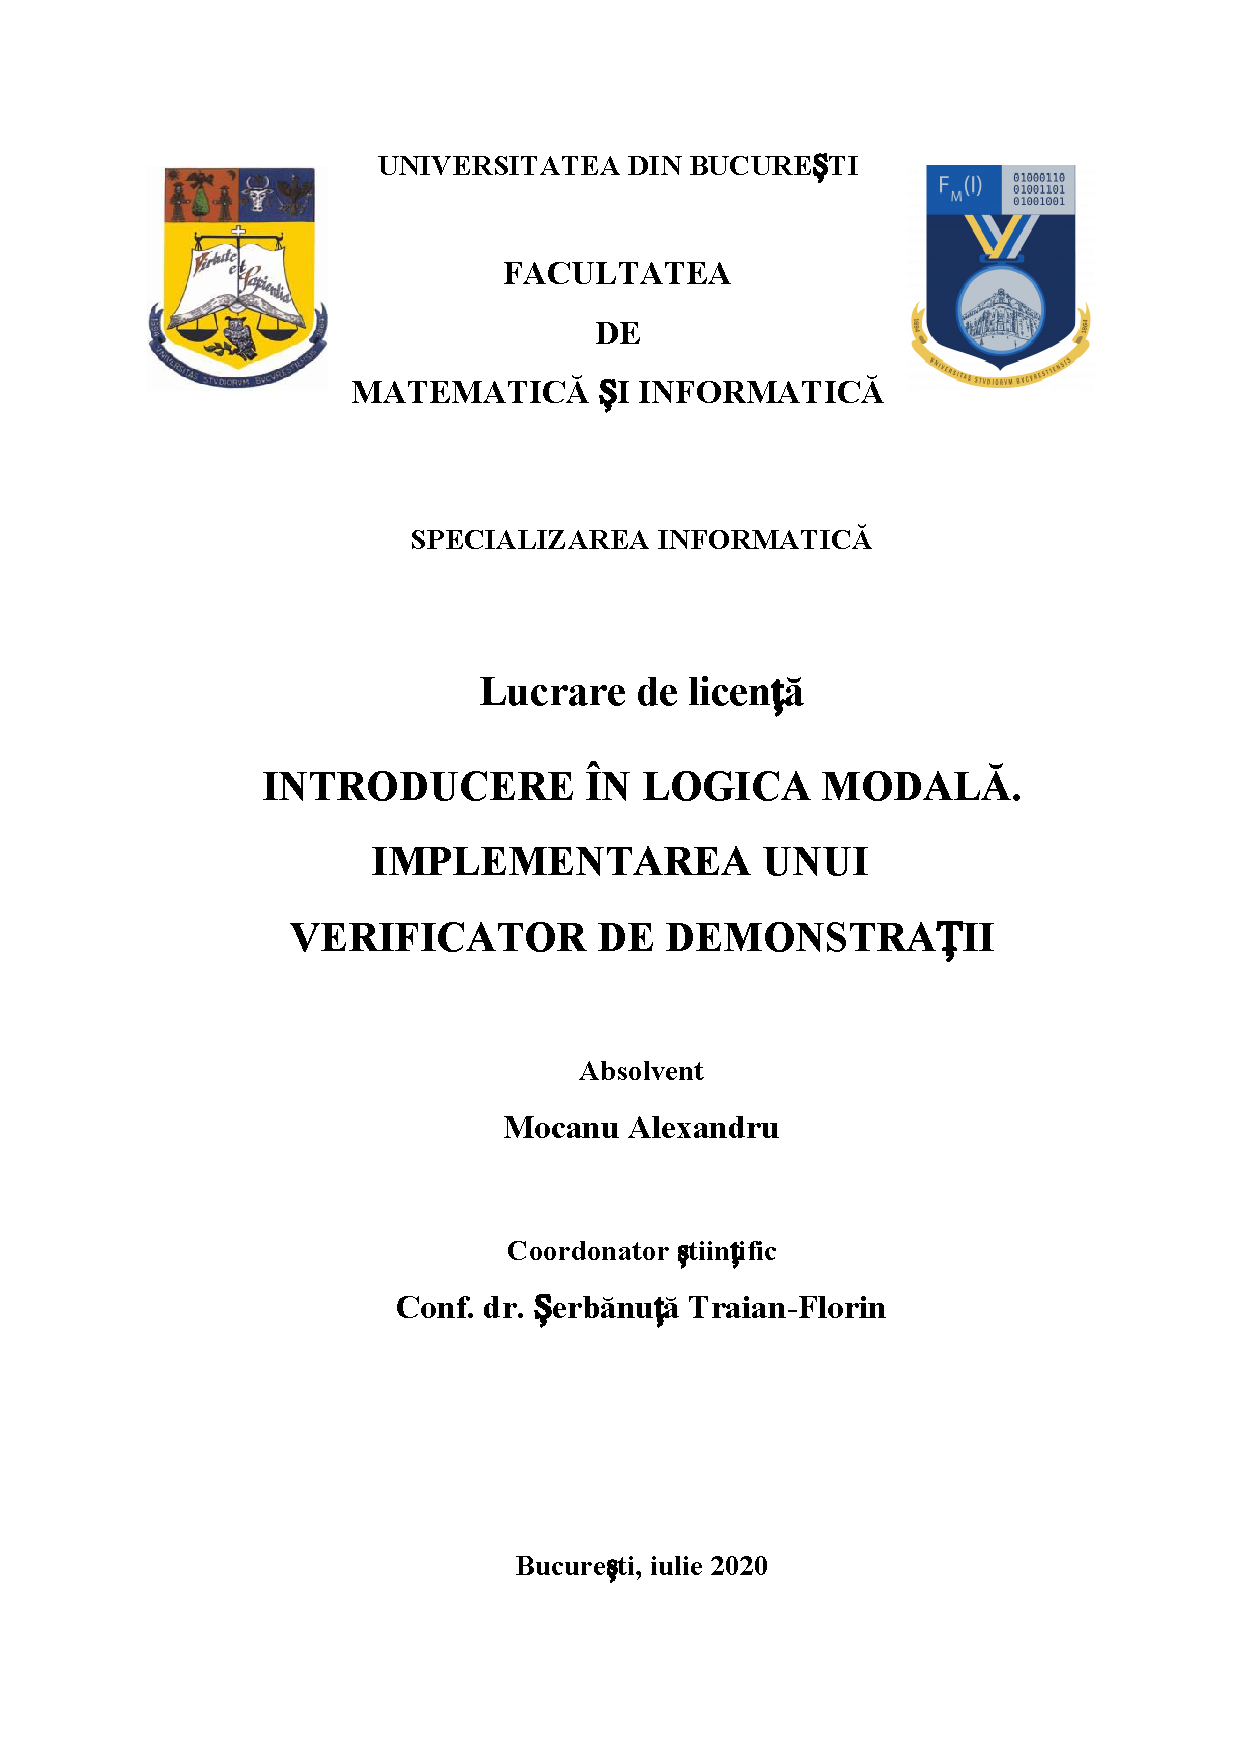
\includepdf[page={1}]{images/first_page.pdf}


    \par{}
    \centerline{\Large \textbf{Rezumatul lucrării}}
    \vspace{20pt}
        Această lucrare este adresată în principal studențiilor sau, în general, persoanelor care doresc să descopere 
        bazele logicii modale. În prima parte a acestei lucrări, sunt sintetizate noțiunile cele mai comune, plecând de 
        la elementele de sintaxă și semantică și ajungând la demonstrațiile sintactice. Toate acestea sunt însoțite
        de exemple menite să ilustreze conceptele prezentate, dar și să arate principalele utilizări ale logicii modale, 
        precum și diversitatea acestora. La sfârșitul acestei părți, cititorul ar trebui să poată înțelege puterea de 
        modelare pe care o oferă această logică. Mai mult decât atât, partea a doua a acestei lucrări dorește să 
        nuanțeze legătura dintre conceptele logice și programare, prin implementarea unui verificator de demonstrații 
        pentru logica modală de bază, sub forma unui modul de Haskell denumit ModalProofChecker. Acesta are atât un rol 
        practic putând fi utilizat pentru a verifica demonstrații realizate pentru logica modală de bază, cât și un rol 
        didactic ilustrând modul în care pot fi utilizate conceptele logice teoretice în cadrul programelor.
    
    \vspace{100pt}
    \par{}
    \centerline{\Large \textbf{Paper abstract}}
    \vspace{20pt}
        This paper is mainly addresed to students or, in general, to any person who wishes to discover the basics of 
        modal logic. The first part of this paper is synthesizing the most common notions, starting with the synthax and 
        semantic elements and reaching the synthactic proofs. All of these are accompanied by examples which are 
        designed to illustrate the presented concepts, but also to show the main use cases of modal logic, as well as 
        their diversity. By the end of this part, the reader should be able to understand the power of modelling that 
        this logic has to offer. More than that, the second part of this paper wishes to emphasize the connection 
        between the logic concepts and programming, by implementing a proof checker for basic modal logic, presented as 
        a Haskell module entitled ModalProofChecker. This one has not only a practical role by being used for checking 
        proofs made in basic modal logic, but also an academic role by showing a way in which the theoretical logic 
        concepts can be used in the context of programs.
    
    \clearpage

    \begingroup
        \let\cleardoublepage\clearpage
        \tableofcontents
        \thispagestyle{empty}
    \endgroup

    \addtocontents{toc}{\protect\thispagestyle{empty}} % Foloseste pentru ToC de mai mult de o pagina
    
    
    \pagestyle{plain}

    \chapter{Introducere} % (fold)
    \label{chapter_introduction}
        \section{Contextul domeniului} % (fold)
        \label{section_context}
            \par{}
                În viața de zi cu zi, se întâmplă adesea ca cineva să considere că o afirmație este adevărată, fără a se 
                îndoi de aceasta, chiar dacă nu este bazată pe un raționament. Astfel de presupuneri pot conduce la 
                deducția altor raționamente greșite. De aceea, în mod natural, apare necesitatea unei modalități mai 
                riguroase decât părerile personale pentru a stabili dacă o afimație este adevărată sau nu. Însă, pentru 
                a putea realiza astfel de raționamente, nu a putut fi folosit limbajul natural din cauza ambiguității pe 
                care o prezintă în anumite contexte, fiind nevoie de o altă modelare a afirmațiilor. Pe aceste 
                considerente, s-a dezvoltat domeniul de studii cunoscut astăzi sub denumirea de logică. Acesta are o 
                istorie foarte îndelungată, bazele sale fiind puse încă din antichitate în secolul 4 î.Hr. de filozoful 
                grec, Aristotel. Deși încă de atunci au fost descoperite moduri de a face inferențe, acestea 
                au reprezentat doar începutul unui drum lung către dezvoltarea unui sistem formal, logica necunoscând 
                schimbări fundamentale până în secolul 17 când Leibniz a realizat că este necesară o conexiune între 
                teoria inferențelor și tipurile de raționamente deductive utilizate în matematică 
                \cite{introduction_to_logic}. Această idee a inspirat mai târziu și alți logicieni precum Boole care a 
                introdus algebra booleană la mijlocul secolului 19 care a reprezentat bază matematică pentru 
                componentele hardware, cât și pentru logica propozițională \cite{logic_computer_science}. În final, 
                acestea au culminat la începutul secolului trecut cu realizarea sistemelor de deducție datorită muncii 
                multor logicieni și matematicieni, dintre care probabil cei mai importanți au fost Frege, Peano, 
                Russell, Kurt G\unichar{"00F6}del, David Hilbert și Alfred Tarski \cite{introduction_to_logic}. Acestea 
                sunt astăzi utilizate în diverse tipuri de logici, precum și în logica modală.
            
            \par{}
                Logica modală este referită de multe ori sub denumirea de „logica posibilități și necesității”, prin 
                expresie modală înțelegându-se un mod de a califica adevărul în raționamente 
                \cite{stanford_modal_logic}. Motivația apariției acestui tip de logică este legată de necesitatea de a 
                avea mai multe „tipuri” de adevăr („posibil adevărat”, „se crede că este adevărat”, „este necesar să fie
                adevărat”). Acesta a fost introdus prima dată de C.I. Lewis în lucrarea 
                \textit{Survey of Symbolic Logic} publicată îm anul 1918, care a extins logica propozițională printr-un 
                operator modal unar I ce semnifica „este imposibil ca”. Un alt moment important în istoria logicii 
                modale este marcat de introducerea elementelor semantice precum conceptele de \textit{frame} și model ce 
                au permis rezolvarea unor probleme dificile până la acel moment \cite{modal_logic}. În contextul actual, 
                logica modală cunoaște o creștere foarte accelerată, fiind dezvoltate multe \textit{tool}-uri pentru 
                diverse aplicații în domeniu. Probabil cel mai de interes dintre acestea sunt demonstratoarele automate 
                de teoreme \myenglishterm{automated theorem prover, ATP} care au cunoscut diverse abordări. Câteva 
                exemple de astfel de programe sunt KSP, MLTP și MleanCop, care este implementat pentru a suporta și 
                operatorii din logica de ordinul întâi \cite{ksp}\cite{mltp}\cite{MleanCop}. Însă problema este una 
                complexă și multe sisteme ajung să renunțe la performanță pentru a crește gradul de generalitate. Pe de 
                altă parte, o altă abordare a fost de a restrânge cerințele în dorința de a se rezolva o problemă mai 
                specifică, dar cu o performanță sporită. Un astfel de exemplu este KeYmaera X care este axat pe 
                verificarea corectitudinii programelor, folosind logica dinamică \cite{KeYmaera}.
        % section Contextul domeniului (end)

        \section{Descrierea lucrării} % (fold)
        \label{section_description}
            \par{}
                Logica modală este un subiect foarte vast care a condus și la apariția multor altor sisteme logice 
                bazate pe conceptele sale. În plus, gradul de generalitate pe care îl conferă permite modelarea 
                multor probleme diverse. Acest lucru poate fi rezumat de un citat din cartea „Modal Logic”: \textit{„once 
                you get to the end of the book, you will discover that far from having learned everything about modal 
                logic, you have merely arrived at the beginning of an unending journey...}” („când vei ajunge la 
                sfârșitul acestei cărți, vei descoperi că te afli departe de a fi învățat totul despre logica modală, ci 
                te afli abia la începutul unei călători fără sfârșit...”) \cite{modal_logic}.
            
            \par{}
                De aceea, acest domeniu poate părea greu de pătruns de cineva ce are doar cunoștințe de bază în ceea ce 
                privește logica. Acesta este problema principală ce se dorește a fi abordată în această lucrare, o 
                prezentare a logicii modale care să fie accesibilă cât mai multor persoane. Aceasta nu înseamnă că se 
                dorește o renunțare la definiții formale sau demonstrații riguroase, ci că se urmărește construirea unei
                intuiții pe baza acestora. În plus, în a doua parte a lucrării, se vrea nuanțarea importanței practice 
                pe care o are acest domeniu. Exemplul practic prezentat nu este o inovație pentru logica modală, prin 
                prezentarea sa dorindu-se mai mult a se arăta că noțiunile prezentate nu reprezintă doar concepte 
                abstracte, fiind ilustrat un mod în care acestea pot fi modelate și utilizate în cadrul unui program. În 
                ceea ce privește punctele ce se doresc a fi atinse în implementarea verificatorului de demonstrații 
                trebuie menționate claritatea modelării conceptelor (acestea trebuie să fie ușor de înțeles), 
                specificarea detaliată a erorilor apărute de-a lungul unei demonstrații și, nu în ultimul rând, ușurința 
                de utilizare a acestuia.
        % section Descrierea lucrării (end)

        \section{Structura lucrării} % (fold)
        \label{section_structure}
            \par{}
                Acum că obiectivele acestei lucrări sunt clare, va fi prezentată structura lucrării pentru a ilustra 
                și modul în care vor fi atinse aceste obiective. În \mysectionreference{chapter_modal_logic}, sunt 
                introduse conceptele cele mai imporante din logica modală. În secțiunea 1, este prezentată o 
                motivație a necesității logicii modale. Apoi, în secțiunile 2, 3 și 5 sunt definite noțiunile 
                de bază ale logicii modale ce includ elementele de sintaxă și semantică, cât și conceptele de 
                satisfiabilitate și validitate a formulelor. Secțiunea 4 a capitolului este rezervată prezentării 
                câtorva exemple care ilustrează puterea de modelare oferită de logica modală. Mai departe, în secțiunile 
                6 și 7 sunt definite demonstrațiile sintactice fiind utilizate sisteme de tip Hilbert. Pentru a 
                introduce gradual elementele noi din logica modală, primele șapte secțiuni fac doar trimiteri la logica 
                modală de bază, generalizarea acesteia realizându-se în secțiunea 8. Aceasta are și rolul de a 
                prezenta și câteva exemple mai complexe ce pot fi modelate cu ajutor logicii modale. Definițiile și 
                propozițiile prezentate sunt o sinteză a multor rezultate deja consacrate ce se regăsesc în cartea 
                „Modal Logic” scrisă de Patrick Blackburn, Maarten de Rijke și Yde Venema \cite{modal_logic}, precum și 
                în alte publicații ce abordează această tematică. În \mysectionreference{chapter_demonstration_checker}, 
                discuția este dedicată detaliilor implementării modulului \textbf{ModalProofChecker}, realizat în 
                Haskell, ce oferă funcționalitate pentru verificarea demonstrațiilor ce utilizează logica modală de 
                bază. În primele două secțiuni sunt descrise în detaliu seminificația unui verificator, respectiv limbajul 
                de programare utilizat și avantajele conferite de acesta. Secțiunea 3 prezintă modul în care au fost 
                modelate conceptele necesare din logica modală, iar secțiunea 4 descrie implementarea efectivă a 
                verificatorului de demonstrații. Ultima secțiune a acestui capitol oferă detalii pentru utilizarea 
                modulului ce sunt ilustrate prin exemple. Modulul \textbf{ModalProofChecker} prezentat în acest capitol 
                reprezintă contribuția personală a autorului. În ultimul capitol, 
                \mysectionreference{chapter_conclusion}, este realizată o apreciere critică menită să stabilească cât de 
                bine a reușit această lucrare să și atingă obiectivele. În plus, sunt prezentate și posibile 
                îmbunătățiri ale lucrării.
            
            \par{}
                Un alt fapt ce trebuie menționat este legat de cunoștințele pe care trebuie să le aibă o persoană 
                pentru a putea înțelege cât mai bine ideile prezentate în această lucrare. Din acest punct de vedere, 
                \mysectionreference{chapter_modal_logic} nu necesită nici o cunoștință legată de logica modală, fiind o
                introducere în acest domeniu. Cu toate acestea, ținând cont de faptul că logica modală este o extensie a 
                logicii propoziționale, este necesar să se fi studiat anterior aceast tip de logică chiar și la un nivel 
                de bază. O cunoaștere bună a logicii propoziționale va conduce automat la o înțelegere mai ușoară a 
                conceptelor din logica modală. În ceea ce privește \mysectionreference{chapter_demonstration_checker}, 
                din punct de vedere teoretic, trebuie să fie parcurs capitolul anterior pentru a putea înțelege atât 
                implementarea, cât și utilitatea exemplului practic. Implementarea acestuia este descrisă în detaliu 
                astfel încât structura utilizată poate fi înțeleasă și fără a se cunoaște particularități ale limbajului 
                Haskell sau ale programării funcționale, totuși, sunt necesare cunoștințe de bază de programare. Pe de 
                altă parte, limbajul Haskell este o cerință pentru o înțelegere completă a exemplului, fiind necesare 
                chiar și concepte mai avansate precum monadele. În plus, având în vedere că funcționalitatea 
                implementată este încapsulată într-un modul de Haskell, este evident necesară cunoașterea limbajului 
                pentru a putea utiliza produsul dezvoltat.
        % section Structura lucrării (end)
    % chapter Introducere (end)

    \chapter{Logică Modală} % (fold)
    \label{chapter_modal_logic}
        \section{Introducere în logica modală} % (fold)
        \label{section_intro_modal}
            \par{}
                În logica propozițională și în logica de ordinul întâi, formulele sunt interpretate doar ca 
                fiind adevărate sau false, fără a putea fi evaluate din punct de vedere calitativ sau contextual.
                Însă, de multe ori, este necesar să existe și posibilitatea unei interpretări a expresiilor 
                în timp sau în funcție de ipostaza în care se află un sistem. Acest lucru este formalizat 
                în cadrul logicii modale prin utilizarea stărilor. Introducerea acestora conservă generalitatea 
                sistemul logic, deoarece interpretarea semnificației acestor stări poate fi diversă. De asemenea, 
                logica modală introduce expresii precum \textit{este necesar să fie adevărat}, \textit{va 
                fi întotdeauna adevărat}, \textit{se știe că este adevărat} sau \textit{se crede că este adevărat}
                \cite{lecture_notes_hedin}. Spre exemplu, afirmația \\\\
                \centerline{\textit{„Uniunea Europeană este constituită din 27 state membre.”}} \\\\
                este adevărată în luna iunie a anului 2020. Totuși, aceasta nu reprezintă un adevăr ce persistă în 
                timp, având în vedere că alte state pot adera ulterior. Pe de altă parte, în analiza propoziției 
                \\\\ \centerline{\textit{„Singurul număr prim par este 2.”}} \\\\
                se distinge o afirmație care este adevărată în acest moment, dar care va continua să fie adevărată
                și în viitor.
        % section Introducere (end)

        \section{Sintaxa} % (fold)
        \label{section_synthax}
            \par{}
                În această secțiune este ilustrat cum arată o expresie în logica modală, cum se definește o 
                formulă bine formată și cum putem descrie mulțimea formulelor logice. Pentru a defini aceste formule, 
                se pornește de la o mulțime de propoziții atomice, similară celei folosite în 
                logica propozițională și în logica de ordinul întâi. În cele ce urmează, se notează această mulțime 
                cu $Prop$.
            
            \begin{definition}
            \label{def_basic_synthax}
                O formulă a logicii modale de bază $\varphi$ este o expresie peste mulțimea simbolurilor $Prop 
                \cup \{\bot, \top, \neg, \vee, \wedge, \rightarrow, \leftrightarrow, \Box, \Diamond, (, )\}$, care 
                respectă una din următoarele reguli:
                \begin{itemize}
                    \item $\varphi \in Prop \cup \{\bot, \top\}$ (este o propoziție atomică, adevărul 
                    sau falsul)
                    \item $\varphi = \chi \vee \psi, unde\: \chi,\psi$ sunt formule (este o disjuncție între două 
                    formule)
                    \item $\varphi = \chi \wedge \psi, unde\: \chi,\psi$ sunt formule (este o conjuncție între 
                    două formule)
                    \item $\varphi = \chi \rightarrow \psi, unde\: \chi,\psi$ sunt formule (este o implicație 
                    în care premisa și concluzia sunt formule)
                    \item $\varphi = \chi \leftrightarrow \psi, unde\: \chi,\psi$ sunt formule (este o echivalență 
                    între două formule)
                    \item $\varphi = \neg \chi, unde\: \chi$ este formulă (este negația unei formule)
                    \item $\varphi = \Box \chi\: sau\: \varphi = \Diamond \chi, unde\: \chi$ este formulă (pătratul 
                    și diamantul sunt operatori specificii logicii modale, al căror comportament va fi detaliat 
                    ulterior)
                \end{itemize}
            \end{definition}

            \par{}
                Se observă că definiția formulelor pentru logica modală nu diferă foarte mult față de 
                logica propozițională. Singurele elemente de noutate, care apar în această definiție, sunt cei 
                doi operatori, pătrat și diamant. Sintactic, este importantă dualitatea dintre cei 
                doi operatori. Din acest punct de vedere, $\Box\; și\; \Diamond$ se 
                aseamănă foarte mult cu operatorii logicii de ordinul întâi, $\forall\; și\; \exists$.
        % section Sintaxa (end)

        \section{Semantica}
        \label{section_semantics}
            \par{}
                Din perspectiva semantică, logica modală începe să difere semnificativ 
                față de sistemul logicii propoziționale, deoarece este necesară o structură care să permită 
                evaluarea diferită a unei expresii în funcție de un context. Astfel, apar două noi concepte strâns 
                legate între ele, și anume conceptul de \textit{frame} și cel de model Kripke.
            
            \begin{definition}
                Un \textit{frame} pentru logica modală de bază este o pereche $\mathcal{F} = (W, R)$, unde:
                \begin{enumerate}
                    \item W este o mulțime nevidă
                    \item R este o relație binară peste W, $R \subseteq W \times W$
                \end{enumerate}
            \end{definition}

            \par{}
                Dintr-o perspectivă mai intuitivă, mulțimea W este mulțimea stărilor, denumite și lumile \textit{frame}-ului. 
                Relația R este cea care creează legăturile între aceste lumi. Dacă $(w_1, w_2) \in R$, se spune că lumea $w_2$ 
                este accesibilă din lumea $w_1$. Fără aceste legături, totul s-ar reduce la modelul logicii propoziționale, 
                fiecare afirmație fiind evaluată într-o lume ținând cont doar de contextul lumii respective și nu de cum se 
                poziționează aceasta față de celelalte lumi. 
            
            \begin{example}
                O utilizare des întâlnită a logici modale este definirea mulțimii W ca fiind formată din stările 
                prin care trece un sistem la diverse momente de timp și a lui R ca fiind relația care ordonează 
                cronologic aceste stări. Astfel, o lume $w_2$ este accesibilă dintr-o altă lume $w_1$ doar dacă 
                $w_2$ corespunde unui moment de timp ulterior celui corespunzător lui $w_1$.
            \end{example}
            
            \par{}
                Însă acest exemplu nu este singura interpretare posibilă, această definiție a \textit{frame}-urilor 
                permițând modelarea tuturor sistemelor la baza cărora se află o structură de graf \cite{handbook_modal_logic}.

            \par{}
                Conceptul de \textit{frame}, deși prezintă structura unui sistem de logică modală, nu oferă informații 
                calitative pentru interpretarea expresiilor. Pentru a putea stabili o valoare de adevăr pentru expresii, 
                avem nevoie de o funcție de evaluare, similară celei din logica propozițională, dar care să țină cont și de
                structura logicii modale. Astfel, se introduce modelul Kripke, denumit astfel după Saul Kripke, cel care l-a 
                introdus în anii 1950 \cite{lecture_notes_hedin}.
            
            \begin{definition}
                Un model pentru logica modală de bază este o pereche $\mathcal{M} = (\mathcal{F}, L)$, unde:
                \begin{enumerate}
                    \item $\mathcal{F} = (W, R)$ este un \textit{frame}
                    \item L este o funcție de evaluare \myenglishterm{labelling function},
                    $L : W \rightarrow \mathcal{P}(Prop)$
                \end{enumerate}
            \end{definition}

            \par{}
                Se poate observa că un model este doar alăturarea dintre un \textit{frame} și o funcție de evaluare care 
                permite interpretarea expresiilor. Funcția de evaluarea atribuie fiecărei lumii \textit{w} o mulțime de atomi
                propoziționali, cu semnificația că aceștia sunt toți atomii adevărați în lumea \textit{w}. Este important
                de menționat faptul că, în contextul unui model $\mathcal{M} = (\mathcal{F}, L)$, se spune că $\mathcal{M}$ 
                este bazat pe \textit{frame}-ul $\mathcal{F}$ sau că \textit{frame}-ul $\mathcal{F}$ stă la baza lui 
                $\mathcal{M}$.

            \par{}
                Odată fixate conceptele de \textit{frame} și model, se poate defini ce înseamnă că o afirmație este adevărată
                în cadrul unei lumi.
            
            \begin{definition}
                Fie un model $\mathcal{M} = ((W, R), L)$ și $x \in W$. Se definește inductiv ce înseamnă că o formulă 
                este adevărată în lumea x sau ce înseamnă că x satisface o formulă (se notează cu $\mathcal{M},x \Vdash 
                \varphi$, unde $\varphi$ este o formulă):
                \begin{itemize}
                    \item $\mathcal{M},x \Vdash \top$
                    \item $\mathcal{M},x \nVdash \bot$
                    \item $\mathcal{M},x \Vdash v$ dacă și numai dacă $v \in L(x)$
                    \item $\mathcal{M},x \Vdash \neg\varphi$ dacă și numai dacă $\mathcal{M},x \nVdash \varphi$
                    \item $\mathcal{M},x \Vdash \varphi \wedge \chi$ dacă și numai dacă $\mathcal{M},x \Vdash \varphi$ și $\mathcal{M},x \Vdash \chi$
                    \item $\mathcal{M},x \Vdash \varphi \vee \chi$ dacă și numai dacă $\mathcal{M},x \Vdash \varphi$ sau $\mathcal{M},x \Vdash \chi$
                    \item $\mathcal{M},x \Vdash \varphi \rightarrow \chi$ dacă și numai dacă $\mathcal{M},x \Vdash \chi$ când $\mathcal{M},x \Vdash \varphi$
                    \item $\mathcal{M},x \Vdash \varphi \leftrightarrow \chi$ dacă și numai dacă $\mathcal{M},x \Vdash \varphi$ dacă și numai dacă 
                    $\mathcal{M},x \Vdash \chi$
                    \item $\mathcal{M},x \Vdash \Box\varphi$ dacă și numai dacă pentru orice $y \in W$ cu $(x,y) \in R$ are loc $\mathcal{M},y \Vdash \varphi$ 
                    \item $\mathcal{M},x \Vdash \Diamond\varphi$ dacă și numai dacă există $y \in W$ cu $(x,y) \in R$ pentru care are loc $\mathcal{M},y \Vdash \varphi$
                \end{itemize}
            \end{definition}

            \par{}
                Adaptând definiția din logica propozițională (ce înseamnă că o expresie este adevărată) folosind funcția de evaluare din logica modală,
                se obține definiția de mai sus, exceptând operatorii $\Box$ și $\Diamond$ (deoarece aceștia nu apar în logica propozițională). 
                Așadar, noutatea care se remarcă în acestă definiție este dată de modalitatea prin care sunt evaluați operatorii $\Box$ 
                și $\Diamond$. Se poate observa că acești operatori sunt introduși pentru a realiza conexiunile dintre lumi. 
                Este notabil și faptul că, deși evaluarea celor doi operatori este bine definită, aceasta permite interpretarea 
                operatorilor în diverse moduri. Acest lucru va fi detaliat și exemplificat ulterior.
        % section Semantica (end)

        \section{Interpretări ale logicii modale} % (fold)
        \label{section_engineering}
            \par{}
                După cum a fost prezentat și anterior, logica modală conferă flexibilitate sporită, permițând modelarea multor
                probleme diverse, folosind la bază același sistem. Acest lucru este realizat oferind interpretări diferite 
                celor doi operatori specifici logicii modale, pătratul și diamantul. În continuare, vor fi introduse exemple
                pentru o mai bună înțelegere a acestui concept, în care se observă cum aceeași formulă logică simbolizează
                diferite tipuri de adevăr sub interpretări diferite. De asemenea, se ilustrează în aceste exemple și dependența
                dintre interpretările celor doi operatori duali.

            \par{}
                Se consideră următoarele trei cazuri uzuale pentru interpretarea formulei $\Box\varphi$ \cite{lecture_notes_hedin}:
                \begin{itemize}
                    \item Este necesar ca $\varphi$ să fie adevărată.
                    \item Întotdeauna $\varphi$ va fi adevărată.
                    \item Agentul A știe $\varphi$.
                \end{itemize}
                Pornind de la aceste interpretări ale operatorului pătrat, se vor analiza cum sunt influențate interpretarea 
                operatorului diamant și semnificația lumilor din fiecare caz.

            \par{}
                Pentru început, se va determina interpretarea operatorului diamant, în fiecare dintre cele trei cazuri prezentate.
                Acest lucru este realizat utilizând proprietatea de dualitate a operatorilor pătrat și diamant. Mai precis,
                utilizând relația $\Diamond\varphi := \neg\Box\neg\varphi$, se ajunge la următoarele interpretări 
                pentru formula $\Diamond\varphi$ \cite{lecture_notes_hedin}:
                \begin{itemize}[itemsep=3pt]
                    \item Nu este necesar ca $\neg\varphi$ să fie adevărată. \\
                        $\Leftrightarrow$ Este posibil ca $\neg\neg\varphi$ să fie adevărată. \\
                        $\Leftrightarrow$ Este posibil ca $\varphi$ să fie adevărată.
                    \item Nu întotdeauna $\neg\varphi$ va fi adevărată. \\
                        $\Leftrightarrow$ Într-un moment din viitor, $\neg\neg\varphi$ va fi adevărată. \\
                        $\Leftrightarrow$ Într-un moment din viitor, $\varphi$ va fi adevărată.
                    \item Agentul A nu știe $\neg\varphi$. \\
                        $\Leftrightarrow$ Cunoștințele agentului A sunt consistente (nu intră în contradicție) cu $\neg\neg\varphi$. \\
                        $\Leftrightarrow$ Cunoștințele agentului A sunt consistente (nu intră în contradicție) cu $\varphi$.
                \end{itemize}
                \vspace{6pt}

            \par{}
                Pentru a avea o imagine de ansamblu, trebuie punctat și cum influențează interpretarea 
                operatorului pătrat semnificația relației dintre lumi. Analizând cele trei cazuri prezentate anterior,
                se pot observa următoarele interpretări corespunzătoare pentru relația $(x,y) \in R$ \cite{lecture_notes_hedin}:
                \begin{itemize}
                    \item y este o lume posibilă ținând cont de informația din lumea x.
                    \item Lumea/Starea y este situată cronologic după lumea/starea x.
                    \item y este o lume posibilă conform cunoștințelor agentului A în lumea x.
                \end{itemize}
        % section Interpretări ale logicii modale (end)

        \section{Satisfiabilitate și validitate} % (fold)
        \label{section_satisfiability_validity}
            \par{}
                A fost definit în \mysectionreference{section_semantics} ce înseamnă ca o 
                formulă să fie adevărată în contextul unui model și al unei lumi stabilite. Însă acest lucru nu este 
                suficient, de multe ori fiind necesar să se poată exprima și adevăruri care au un grad mai larg de răspândire.
                Cu alte cuvinte, este de dorit să se poată spune despre o anumită afirmație că este adevărată în orice lume a unui
                model. Astfel, plecând de la definiția existentă, se construiesc următoarele definiții prin generalizare:

            \begin{definition}
                Fie $\mathcal{M} = ((W,R), L)$ un model și $\varphi$ o formulă. Se spune că formula $\varphi$
                este universal adevărată în modelul $\mathcal{M}$, dacă este adevărată relația $\mathcal{M},x \Vdash \varphi$ pentru
                orice $x \in W$. Acest lucru se notează astfel: $\mathcal{M} \Vdash \varphi$.
            \end{definition}

            \begin{definition}
                Fie $\mathcal{M} = ((W,R), L)$ un model și $\varphi$ o formulă. Se spune că formula $\varphi$
                este satisfiabilă în modelul $\mathcal{M}$, dacă există o lume $x \in W$ pentru care este adevărată relația $\mathcal{M},x \Vdash \varphi$.
            \end{definition}

            \begin{example}
            \label{ex_truth_sat}
                Se consideră următoarele mulțimi:
                \begin{itemize}
                    \item $W=\{w_1, w_2, w_3, w_4\}$
                    \item $R=\{(w_1, w_2), (w_1, w_3), (w_2, w_4), (w_3, w_4)\}$
                    \item $L(w_1)=\oslash,\; L(w_2)=\{p,q,r\},\; L(w_3)=\{q,r,s\},\; L(w_4)=\{q,s\}$
                \end{itemize}

                \begin{figure}[h!]
                \label{fig_example_1}
                    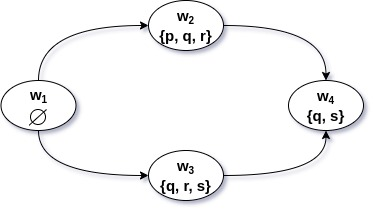
\includegraphics[width=0.5\linewidth]{images/example_1.jpg}
                    \centering
                    \caption{Reprezentare grafică a exemplului \ref{ex_truth_sat}}
                \end{figure}
                \vspace{101pt}
                
                Analizând modelul $\mathcal{M}=(\mathcal{F},L)$, se constată următoarele:
                
                \begin{itemize}
                    \item Este adevărată relația $\mathcal{M},w_1 \Vdash \Diamond p \wedge \Diamond s$, deoarece avem 
                    $\mathcal{M},w_2 \Vdash p$ ($w_2$ este accesibilă din $w_1$) și $\mathcal{M},w_3 \Vdash s$ ($w_3$ este 
                    accesibilă din $w_1$). Însă, se remarcă și faptul că formula $\Diamond (p \wedge s)$ nu este adevărată 
                    în lumea $w_1$, deoarece nici în $w_2$, nici în $w_3$, nu este adevărată formula $p \wedge s$. Acest lucru
                    relevă o proprietate mai generală: $\Box$ nu este distributivă față de $\vee$, iar $\Diamond$ nu este 
                    distributivă față de $\wedge\;$\cite{lecture_notes_hedin}. De asemenea, se poate arăta că $\Box$ este 
                    distributivă față de $\wedge$, iar $\Diamond$ este distributivă față de $\vee$.
                    \item Formula $p \wedge s$ nu este satisfiabilă în acest model, deoarece nu avem nici o lume în care să 
                    fie adevărate atât p, cât și s.
                    \item Este adevărat că $\mathcal{M},w_1 \Vdash \Box r$, deoarece $w_2$ și $w_3$ sunt singurele lumi 
                    accesibile din lumea $w_1$, iar în ambele este adevărată propoziția r.
                    \item Formula $\Box q$ este universal adevărată în model ($\mathcal{M} \Vdash \Box q$). Folosind un 
                    raționament similar celui de la subpunctul anterior, se demonstrează că formula este adevărată în lumile
                    $w_1, w_2$ și $w_3$. Pentru $w_4$, formula $\Box q$ este adevărată, deoarece nu există nici o lume accesibilă din $w_4$.
                    Aceste tipuri de lumi sunt denumite \textit{dead ends} și toate formulele de forma $\Box \varphi$ sunt 
                    adevărate în aceste lumi \cite{modal_logic}. În plus, toate formulele de forma $\Diamond \varphi$ sunt 
                    false în aceste lumi.
                \end{itemize}
            \end{example}

            \par{}
                Conceptul de satisfiabilitate se referă la adevărul doar pentru o anumită evaluare, dar, similar cu logica 
                propozițională, se poate vorbi despre o altă noțiune importantă, și anume validitatea. Aceasta este o generalizare
                a satisfiabilități, întrucât în acest caz raportarea nu se mai realizează la un anumit model, ci la un \textit{frame},
                la toate \textit{frame}-urile (în general) sau, după cum va fi prezentat și în 
                \mysectionreference{section_frame_classes}, la o clasă de \textit{frame}-uri.

            \begin{definition}
                Se spune despre o formulă $\varphi$ că este validă în contextul unei stări w din cadrul unui \textit{frame} 
                $\mathcal{F}$, dacă este adevărată pentru toate modelele $\mathcal{M}=(\mathcal{F}, L)$ ($\mathcal{M},w \Vdash \varphi$),
                unde L este o funcție de evaluare. Acest lucru se notează astfel: $\mathcal{F},w \vDash \varphi$.
            \end{definition}

            \begin{definition}
                Se spune despre o formulă $\varphi$ că este validă în cadrul unui \textit{frame} $\mathcal{F}$, dacă este 
                validă pentru toate stările din $\mathcal{F}$ ($\mathcal{F},w \vDash \varphi$, pentru oricare $w \in W$). 
                Acest lucru se notează astfel: $\mathcal{F} \vDash \varphi$.
            \end{definition}

            \par{}
                \noindent \textit{Observație:} Sunt folosite simboluri diferite pentru a realiza distincția dintre cele două concepte
                prezentate, satisfiabilitatea și validitatea.

            \begin{example}
            \label{ex_validity}
                Se consideră:

                \begin{itemize}
                    \item $W=\{1, 2, 3, 4\}$
                    \item $R=\{(1,2), (1,3), (1,4), (2,4)\}$ (relația de divizibilitate pe 
                    mulțimea W între numere strict diferite)
                \end{itemize}

                \begin{figure}[h!]
                    \label{fig_example_2}
                    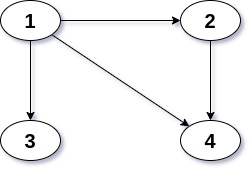
\includegraphics[width=0.5\linewidth]{images/example_2.jpg}
                    \centering
                    \caption{Reprezentare grafică a exemplului \ref{ex_validity}}
                \end{figure}

                Se va demonstra că $\mathcal{F} \vDash \Box \varphi \rightarrow \Box \Box \varphi$, unde $\mathcal{F}=(W,R)$.
                După cum a fost punctat și în exemplul anterior, în cazul stărilor \textit{dead end} (pentru care nu există
                nici o stare accesibilă), toate formulele care încep cu $\Box$ sunt adevărate. Deci, pentru stările 3 și 4 
                se poate concluziona că formula analizată este validă. Rămân de discutat cazul stărilor 1 și 2. 
                \begin{itemize}
                    \item În cazul stării 1: Se presupune că premisa formulei este adevărată ($\Box \varphi$). Deci pentru toate 
                    stările accesibile din 1 (toate stările din W, mai puțin starea 1) formula $\varphi$ este validă. Se 
                    dorește să se arate că formula $\Box \Box \varphi$ este validă în starea 1. Pentru aceasta, este suficient
                    să se arate că formula $\Box \varphi$ este validă în stările 2, 3 și 4. În toate stările, cu excepția 
                    stării 1, formula $\varphi$ este validă. În plus, din nici o stare nu este accesibilă starea 1 
                    ($(x,1) \notin R$, pentru orice x), deci se poate conchide că formula $\Box \Box \varphi$ este validă în
                    starea 1 și deci și formula inițială este validă în starea 1.
                    \item În cazul stării 2: Se arată că formula este validă, deoarece concluzia implicației este totdeauna 
                    adevărată. Pentru ca $\mathcal{F},2 \vDash \Box \Box \varphi$ trebuie ca în toate stările accesibile din 2 
                    să fie validă formula $\Box \varphi$. Singura stare accesibilă din 2 este 4, deci trebuie ca $\mathcal{F}, 4
                    \vDash \Box \varphi$, ceea ce este adevărat folosind același argument pentru stările \textit{dead end}.
                \end{itemize}
                Pentru a finaliza studiul acestui exemplu, se poate concluziona că formula $\Box \varphi \rightarrow \Box 
                \Box \varphi$ este validă în cadrul \textit{frame}-ului analizat.
            \end{example}
            
            \par{}
                \noindent \textit{Observație}: Acesta este doar un rezultat particular care se bazează pe o proprietate mai 
                generală a \textit{frame}-urilor a căror relație de accesibilitate este tranzitivă. Acest cadru mai general 
                va fi prezentat în \mysectionreference{section_frame_classes} alături de alte exemple de astfel de
                proprietăți.

            \par{}
                Un alt caz de validitate care merită menționat este cazul general, cel al formulelor adevărate indiferent de
                structura în care sunt evaluate.

            \begin{definition}
                Se spune despre o formulă $\varphi$ că este validă dacă este validă în toate \textit{frame}-urile 
                ($\mathcal{F} \vDash \varphi$, pentru orice \textit{frame} $\mathcal{F}$). Acest lucru se notează astfel: 
                $\vDash \varphi$.
            \end{definition}

            \begin{sentence}
            \label{prop_axiom_K}
                Formula $\Box (\varphi \rightarrow \psi) \rightarrow (\Box \varphi \rightarrow \Box \psi)$, cunoscută 
                sub denumirea de formula K în onoarea lui Saul Kripke \cite{lecture_notes_hedin}, este validă.   
                
                \begin{proof}[\textbf{Demonstrație:}]
                    Fie $\mathcal{F}$ un \textit{frame} care stă la baza modelului $\mathcal{M}=(\mathcal{F},L)$ și w o stare 
                    din acest \textit{frame}. Se presupune că premisa formulei și premisa concluziei formulei sunt adevărate în 
                    această stare, deci sunt veridice următoarele două afirmații: $\mathcal{M},w \Vdash \Box (\varphi \rightarrow
                    \psi)$ și $\mathcal{M},w \Vdash \Box \varphi$. Din cele două relații se poate deduce că pentru orice stare x
                    accesibilă din starea w trebuie să fie adevărate $\mathcal{M},x \Vdash \varphi \rightarrow \psi$ și 
                    $\mathcal{M},x \Vdash \varphi$. În continuare, folosindu-se regula de evaluare a implicației, se poate deduce
                    că și formula $\psi$ este adevărată în starea x, ceea ce înseamnă că formula $\Box \psi$ este adevărată în 
                    starea w. Urmând înlănțuirea definițiilor anterioare se poate vedea că aceasta este ceea ce se dorea să se 
                    demonstreze, deci se poate conchide că formula K este validă.
                \end{proof}
            \end{sentence}
        % section Satisfiabilitate și validitate (end)

        \section{Clase de \textit{frame}-uri} % (fold)
        \label{section_frame_classes}
            \par{}
                În secțiunea anterioară, a fost prezentată noțiunea de validitate a unei formule, începând de la contextul unei
                stări, apoi continuând cu validitatea în cadrul unui \textit{frame} și, în final, cazul formulelor valide indiferent
                de structura unui \textit{frame}. Ultimele două dintre acestea relevă cazuri interesante de studiat din punct de vedere
                al generalității pe care îl prezintă, însă a fost nevoie de o structură cu un grad intermediar de generalitate, 
                ceea ce a dus la introducerea noțiunii de clase de \textit{frame}-uri \cite{modal_logic}. Aceste clase 
                sunt mulțimi de \textit{frame}-uri care au una sau mai multe proprietăți comune. Așadar, înainte de a prezenta
                mai detaliat clasele de \textit{frame}-uri, trebuie să se definească ce reprezintă o proprietate.

            \begin{definition}
            \label{def_property}
                Se spune despre o formulă $\varphi$ din logica modală că definește o proprietate P a unui \textit{frame} 
                $\mathcal{F}=(W,R)$, dacă $\mathcal{F} \vDash \varphi$ dacă și numai dacă relația R are proprietatea P.
            \end{definition}
            
            \par{}
                În continuare, vor fi prezentate cele mai comune, și totodată importante, proprietăți ale relațiilor de 
                accesibilitate dintre lumi \cite{stanford_modal_logic}:
                \begin{enumerate}
                    \item Formula $\Box \varphi \rightarrow \varphi$, cunoscută și sub denumirea de axioma \textbf{M}, definește 
                    proprietatea de reflexivitate a relației de accesibilitate ($(w,w) \in R$ pentru orice $w \in W$)
                    \item Formula $\Box \varphi \rightarrow \Box \Box \varphi$, cunoscută și sub denumirea de axioma \textbf{4},
                    definește proprietatea de tranzitivitate a relației de accesibilitate (dacă $(w,v) \in R$ și $(v,u) \in R$ 
                    atunci $(w,u) \in R$, pentru orice $w,v,u \in W$)
                    \item Formula $\Box \varphi \rightarrow \Diamond \varphi$, cunoscută și sub denumirea de axioma \textbf{D},
                    definește proprietatea de serialitate a relației de accesibilitate (pentru orice $w \in W$, există $u \in W$
                    astfel încât $(w,u) \in R$)
                    \item Formula $\varphi \rightarrow \Box \Diamond \varphi$, cunoscută și sub denumirea de axioma \textbf{B},
                    definește proprietatea de simetrie a relației de accesibilitate (dacă $(w,v) \in R$ atunci $(v,w) \in R$
                    pentru orice $w,v \in W$)
                    \item Formula $\Diamond \varphi \rightarrow \Box \Diamond \varphi$, cunoscută și sub denumirea de axioma
                    \textbf{5}, definește o relație euclidiană de accesibilitate (dacă $(w,v) \in R$ și $(w,u) \in R$ atunci
                    $(v,u) \in R$, pentru orice $w,v,u \in W$)
                    \item Formula $\Diamond \varphi \rightarrow \Box \varphi$, cunoscută și sub denumirea de axioma \textbf{CD},
                    definește o relație funcțională de accesibilitate (dacă $(w,v) \in R$ și $(w,u) \in R$ atunci $v=u$, pentru
                    orice $w,v,u \in W$)
                    \item Formula $\Box (\Box \varphi \rightarrow \varphi)$, cunoscută și sub denumirea de axioma $\Box$\textbf{M},
                    definește o relație de accesibilitate \textit{shift reflexivă} (dacă $(w,v) \in R$ atunci $(v,v) \in R$, 
                    pentru orice $w,v \in R$)
                    \item Formula $\Box \Box \varphi \rightarrow \Box \varphi$, cunoscută și sub denumirea de axioma \textbf{C4},
                    definește o relație de accesibilitate densă (pentru orice $w,v \in W$ dacă $(w,v) \in R$ atunci există 
                    $u \in W$ pentru care $(w,u) \in R$ și $(u,v) \in R$)
                    \item Formula $\Diamond \Box \varphi \rightarrow \Box \Diamond \varphi$, cunoscută și sub denumirea de 
                    axioma \textbf{C}, definește o relație convergentă de accesibilitate (pentru orice $w,v,x \in W$ dacă 
                    $(w,v) \in R$ și $(w,x) \in R$ atunci există $u \in W$ pentru care $(v,u) \in R$ și $(x,u) \in R$)
                \end{enumerate}
                \vspace{6pt}
            
            \par{}
                \noindent \textit{Observație:} Când se face referire la formulele care descriu proprietăți ale \textit{frame}-urilor,
                acestea au o formă generală. Astfel, când se spune, de exemplu, că formula $\Box \varphi \rightarrow 
                \varphi$ este validă în cadrul unui \textit{frame}, trebuie interpretat că această afirmație este adevărată 
                pentru orice formulă $\varphi$.

            \par{}
                Pentru a ilustra mai bine această noțiune, vor fi prezentate demonstrații pentru proprietățile de reflexivitate (1),
                tranzitivitate (2) și pentru relația euclidiană (5). Ținând cont de definiția \ref{def_property}, relațiile 
                \textbf{(1)-(9)} sunt relații de echivalență. Ca urmare, va fi necesar să se demonstreze, pentru fiecare 
                caz, câte două implicații: \textbf{(a)} dacă formula este validă în \textit{frame}, atunci relația de 
                accesibilitate trebuie să aibă proprietatea dorită; \textbf{(b)} dacă relația de accesibilitate are 
                proprietatea dorită, atunci formula trebuie să fie validă în contextul \textit{frame}-ului.
            
            \begin{figure}[h!]
                \label{fig_example_3}
                \centering
                \begin{subfigure}[h]{0.3\linewidth}
                    \label{fig_reflexivity}
                    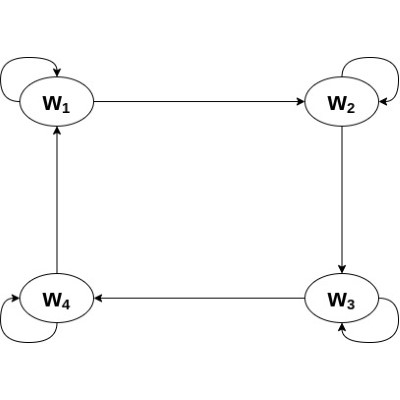
\includegraphics[width=\linewidth]{images/reflexivity.jpg}
                    \caption{Relație reflexivă}
                \end{subfigure}
                \hfill
                \begin{subfigure}[h]{0.3\linewidth}
                    \label{fig_transitivity}
                    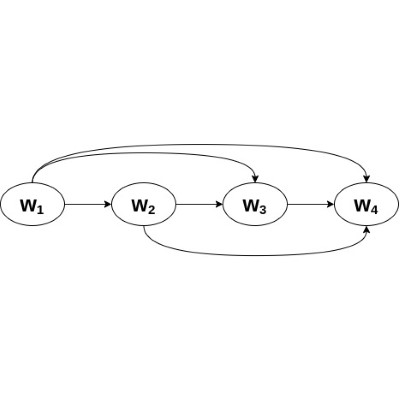
\includegraphics[width=\linewidth]{images/transitivity.jpg}
                    \caption{Relație tranzitivă}
                \end{subfigure}
                \hfill
                \begin{subfigure}[h]{0.3\linewidth}
                    \label{fig_euclidean}
                    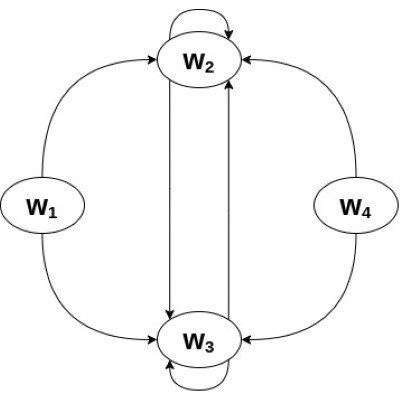
\includegraphics[width=\linewidth]{images/euclidean.jpg}
                    \caption{Relație euclidiană}
                \end{subfigure}
                \caption{Exemple de relații din cele prezentate}
            \end{figure}
            \vspace{76pt}

            \begin{proof}[\textbf{Demonstrație (1):}]
                Pentru implicația \textbf{(a)}, se dorește să se arate că dacă se cunoaște $\mathcal{F} \vDash \Box \varphi 
                \rightarrow \varphi$, unde $\mathcal{F}=(W,R)$ este un \textit{frame}, atunci relația R este reflexivă. 
                Acest caz va fi abordat folosind metoda reducerii la absurd. Așadar, se presupune prin absurd că relația R
                nu este reflexivă și se va construi un model, mai precis o funcție de evaluare, pentru care formula $\Box p 
                \rightarrow p$ nu este adevărată, unde $p \in Prop$ este o propoziție atomică. R nu este o relație 
                reflexivă, atunci înseamnă că există o stare $w \in W$ pentru care $(w,w) \notin R$. Se consideră următorul 
                model $\mathcal{M}=(\mathcal{F},L)$, unde L este o funcție de evaluare, pentru care se definesc: $p \notin 
                L(w)$ și $p \in L(x)$ pentru orice stare x accesibilă din w ($(w,x) \in R$). Se poate observa ușor că 
                această definire a funcției de evaluare este consistentă, datorită faptului că w nu este accesibilă din ea 
                însăși. Acum rămâne doar să se stabilească valorile de adevăr pentru implicația și concluzia formulei 
                inițiale. Din definiția funcției de evaluare decurg natural următoarele rezultate: $\mathcal{M},w \nVdash p$
                și $\mathcal{M},w \Vdash \Box p$, ceea ce conduce la $\mathcal{M},w \nVdash \Box p \rightarrow p$, însă 
                acest lucru intră în contradicție cu presupunerea că formula inițială este validă în acest \textit{frame}. 
                Deci se poate concluziona că relația R este reflexivă.

                Pentru implicația \textbf{(b)}, se presupune că, pentru \textit{frame}-ul $\mathcal{F}=(W,R)$, relația R 
                este reflexivă și se dorește să se arate că afirmația $\mathcal{F} \vDash \Box \varphi \rightarrow \varphi$ 
                este adevărată. Fie $w \in W$ o stare a acestui \textit{frame}, pentru care se știe că $\mathcal{F},w \vDash
                \Box \varphi$, și se urmărește să se ajungă la relația $\mathcal{F},w \vDash \varphi$. Din prima relație 
                rezultă că pentru toate stările $u \in W$ accesibile din starea w se știe că $\mathcal{F},u \vDash \varphi$.
                În plus, deoarece relația R este reflexivă, se cunoaște și faptul că starea w este accesibilă din ea însăși.
                Combinând ultimele două rezultate se obține că $\mathcal{F},w \vDash \varphi$, adică ceea ce se dorea.
            \end{proof}

            \begin{proof}[\textbf{Demonstrație (2):}]
                Similar demonstrației anterioare, se începe cu implicația \textbf{(a)} și se dorește să se arate că dacă 
                $\mathcal{F} \vDash \Box \varphi \rightarrow \Box \Box \varphi$, unde $\mathcal{F}=(W,R)$ este un 
                \textit{frame}, atunci relația R este tranzitivă. Această problemă va fi abordată asemenea prin metoda reducerii 
                la absurd. Se presupune prin reducere la absurd, că relația R nu este tranzitivă, deci că există trei stări
                $w,u,v \in W$ pentru care următoarea relație este adevărată: $(w,u) \in R$ și $(u,v) \in R$, dar $(w,v) 
                \notin R$. Pornind de la această presupunere, se arată că formula anterior menționată nu-și păstrează 
                validitatea pentru o variabilă propozițională $p \in Prop$, lucru care va intra în contradicție cu 
                presupunerea inițială. Se construiește funcția de evaluare L, din cadrul modelului $\mathcal{M}=
                (\mathcal{F},L)$, astfel: $p \notin L(v)$ și $p \in L(x)$ pentru orice stare x cu $(w,x) \in R$ (x 
                accesibilă din w). Din această definiție reies următoarele afirmații $\mathcal{M},w \Vdash \Box p$ și 
                $\mathcal{M},w \nVdash \Box \Box p$ (deoarece v este accesibilă în 2 „pași” din w și $p \notin L(v)$). 
                Așadar, se poate deduce că $\mathcal{M},w \nVdash \Box p \rightarrow \Box \Box p$, deci formula $\Box p 
                \rightarrow \Box \Box p$ nu este validă în \textit{frame}-ul considerat, ceea ce reprezintă o contradicție.

                Pentru sensul invers al echivalenței, cel din implicația \textbf{(b)}, se urmărește demonstrarea faptului că
                într-un \textit{frame} $\mathcal{F}=(W,R)$, a cărui relație de accesibilitate este tranzitivă, formula 
                $\Box \varphi \rightarrow \Box \Box \varphi$ este validă. Se consideră o stare $w \in W$ pentru care se 
                cunoaște $\mathcal{F},w \vDash \Box \varphi$ și se dorește să se demonstreze $\mathcal{F},w \vDash \Box \Box 
                \varphi$. Deci, din prima relație, rezultă că $\mathcal{F},u \vDash \varphi$ pentru orice stare u accesibilă
                din starea w. Pentru a stabili validitatea formulei $\Box \Box \varphi$ în starea w, se consideră o stare $y
                \in W$ accesibilă în doi „pași” din w (există $x \in W$ astfel încât $(w,x) \in R$ și $(x,y) \in R$), dar 
                faptul că relația R este tranzitivă implică existența unei relații directe între starea w și stare y ($(w,y)
                \in R$). Combinând ultimele două rezultate obținute se deduce că $\mathcal{F},y \vDash \varphi$, fapt ce 
                implică imediat și $\mathcal{F},w \vDash \Box \Box \varphi$, adică ceea ce se dorea. Deci se poate conchide că 
                $\mathcal{F},w \vDash \Box \varphi \rightarrow \Box \Box \varphi$.
            \end{proof}

            \begin{proof}[\textbf{Demonstrație (5):}]
                În ceea ce privește implicația \textbf{(a)} a echivalenței, se va dovedi că, dacă într-un \textit{frame} 
                $\mathcal{F}=(W,R)$ este validă formula $\Diamond \varphi \rightarrow \Box \Diamond \varphi$, atunci relația
                de accesibilitate este euclidiană. Urmârind tiparul din demonstrațiile anterioare, și această implicație 
                folosește metoda redurcerii la absurd. Așadar, se presupune că relația R nu este euclidiană, ceea ce 
                înseamnă că există stările $w,u,v \in W$ pentru care sunt adevărate următoarele: $(w,u) \in R$ și $(w,v) \in
                R$, dar $(u,v) \notin R$. Se construiește o funcție de evaluare L, din modelul $\mathcal{M}=(\mathcal{F},L)$
                pentru care formula $\Diamond p \rightarrow \Box \Diamond p$ să nu fie adevărată în lumea w. Pentru aceasta, 
                se construiește funcția L după următoarele reguli: $p \in L(v)$ și $p \notin L(x)$ pentru orice stare $x \in
                W$. Folosind această definiție pentru L se disting următoarele: $\mathcal{M},w \Vdash \Diamond p$ (deoarece 
                v este accesibilă din w și $\mathcal{M},v \Vdash p$) și $\mathcal{M},u \nVdash \Diamond p$ (deoarece singura
                stare în care p este adevărată este v, iar aceasta nu este accesibilă din starea u, conform presupunerii 
                făcute). Din a doua afirmație rezultă că $\mathcal{M},w \nVdash \Box \Diamond p$, deoarece u este accesibilă
                din starea w. Din aceste două rezultate: $\mathcal{M},w \Vdash \Diamond p$, $\mathcal{M},w \nVdash \Box 
                \Diamond p$ se poate deduce că $\mathcal{M},w \nVdash \Diamond p \rightarrow \Box \Diamond p$, ceea ce 
                conduce la o contradicție. Deci relația de accesibilitate R trebuie să fie euclidiană.

                Pentru a arăta implicația \textbf{(b)} a acestei echivalențe, trebuie să se demonstreze că, dacă se consideră
                o relație de accesibilitate euclidiană R a unui \textit{frame} $\mathcal{F}=(W,R)$, atunci formula 
                $\Diamond \varphi \rightarrow \Box \Diamond \varphi$ este validă în contextul lui $\mathcal{F}$. Fie $w \in 
                W$ o stare pentru care se cunoaște că $\mathcal{F},w \vDash \Diamond \varphi$ și se va arată că 
                $\mathcal{F},w \vDash \Box \Diamond \varphi$. Din afirmația anterioară rezultă că există o stare $x \in W$ 
                cu $(w,x) \in R$ pentru care $\mathcal{F},x \vDash \varphi$. Pentru a arăta că formula $\Box \Diamond 
                \varphi$ este validă în starea w, se consideră o stare $y \in W$ pentru care $(w,y) \in R$. Ținând cont că
                starea x și starea y sunt ambele accesibile din starea w și că relația de accesibilitate este euclidiană, se
                deduce că $(y,x) \in R$. Conectând acest rezultat cu $\mathcal{F},x \vDash \varphi$, reiese că 
                $\mathcal{F},y \vDash \Diamond \varphi$. Având în vedere că această afirmație se poate obține pentru orice 
                stare y accesibilă din starea w rezultă că $\mathcal{F},y \vDash \Box \Diamond \varphi$, deci formula 
                $\Diamond \varphi \rightarrow \Box \Diamond \varphi$ este validă.
            \end{proof}

            \par{}
                Clasele de \textit{frame}-uri au un rol foarte important în cadrul demonstrațiilor sintactice, deoarece 
                oferă un criteriu pe baza căruia se poate decide care sunt formulele ce trebuie incluse ca axiome în 
                problema analizată. Împreună cu seminificația simbolurilor $\Box$ și $\Diamond$, descrisă în detaliu în 
                \mysectionreference{section_engineering}, acestea reprezintă principiile care stau la baza 
                alegerii axiomelor pentru demonstrațiile sintactice \cite{lecture_notes_hedin}. 
            
            \begin{example}
                Dacă se modelează o problemă care urmărește evoluția în timp a unui sistem, stările acestuia pot fi 
                considerate momente de timp. Atunci, este de dorit ca relația de accesibilitate, care ordonează 
                cronologic lumile, să aibă proprietatea de tranzitivitate (dacă o stare y este în viitorul unei stări x 
                și o stare z este în viitorul stării y, atunci este natural ca starea z să fie și în viitorul stării x). 
                În plus, în cazurile studierii unor sisteme care funcționează fără oprire, poate fi de dorit și 
                proprieteatea de serialitate (pentru fiecare stare să existe o viitoare stare posibilă).
            \end{example}
        % section Clase de \textit{frame}-uri (end)

        \section{Logici modale normale} % (fold)
        \label{section_normal_modal_logics}
            \par{}
                În această secțiunea, accentul este pus pe demonstrațiile sintactice din cadrul logicii modale. Acestea 
                reprezintă un punct de interes major din perspectiva practică deoarece se pliază cel mai bine pe sistemele 
                de automatizare a demonstrațiilor dezvoltate până în acest moment. Până acum a fost prezentată în 
                \mysectionreference{section_satisfiability_validity} noțiunea de validatate a unei formule care constituie 
                baza demonstrațiilor sintactice, însă acest lucru nu este suficient. 
                Dacă în contextul unui \textit{frame} 
                se poate face pentru fiecare funcție de evaluare o analiză pentru a stabili dacă o formulă este validă sau 
                nu, în contextul unei demonstrații în care se urmărește să se arate că o formulă este validă în orice \textit{frame} sau 
                într-o clasă de \textit{frame}-uri, această 
                abordare nu mai este plauzibilă. Mai mult decât atât, chiar și în contextul unui \textit{frame}, problema 
                poate deveni una dificilă dacă se ia în considerare faptul că mulțimea lumilor poate avea un număr mare de 
                elemente, potențial infinit. Ca urmare, trebuie să se definească riguros o modalitate prin care se poate 
                stabili dacă o formulă este validă.

            \par{}
                Pentru început, se va pleca de la problema validității unei formule într-un context general, abordarea 
                pentru celelalte cazuri dezvoltându-se în jurul acesteia. Pentru obținerea rezultatului dorit, se va 
                construi un sistem axiomatic de tip Hilbert denumit \textbf{K}, acesta fiind sistemul „minimal” folosit 
                pentru a raționa în contextul \textit{frame}-urilor \cite{modal_logic}.

            \begin{definition}
                O \textbf{K}-demonstrație este o secvență de formule, fiecare dintre acestea fiind fie o axiomă, fie 
                se obține din una sau mai multe formule demonstrate anterior aplicând o regulă de deducție 
                \myenglishterm{rule of proof}. Axiomele sistemului \textbf{K} sunt toate tautologiile din logica 
                propozițională, la care se adaugă formula K ($\Box (p \rightarrow q) \rightarrow (\Box p \rightarrow \Box
                q)$) și formula duală ($\Diamond p \leftrightarrow \neg \Box \neg p$), iar regulile de deducție sunt 
                următoarele:
                \begin{itemize}
                    \item \textit{Modus ponens}: dacă se cunoaște $\varphi$ și $\varphi \rightarrow \psi$, atunci se 
                    poate arăta $\psi$
                    \item \textit{Substituția uniformă}: dacă se cunoaște $\varphi$, atunci se poate demonstra $\psi$, 
                    dacă $\psi$ a fost obținută din formula $\varphi$ prin înlocuirea uniformă (a tuturor aparițiilor) a
                    unor propoziții atomice cu formule arbitrare ale logicii modale
                    \item \textit{Generalizarea}: dacă se știe $\varphi$, atunci se deduce $\Box \varphi$               
                \end{itemize}
                O formulă $\varphi$ se numește \textbf{K}-demonstrabilă dacă apare ca ultimă formulă a unei 
                \textbf{K}-demonstrații. Acest lucru se notează astfel: $\vdash_\textbf{K} \varphi$ .
            \end{definition}
            
            \par{}
                \noindent \textit{Observație}: Nu este necesar să se considere toate tautologiile din logica propozițională,
                ci este suficient să se aleagă o submulțime a lor astfel încât toate celelalte să se poată deduce 
                din acestea.

            \par{}
                Noțiunea de \textbf{K}-demonstrație este folosită pentru a arăta că o formulă este validă. Deci un lucru 
                foarte important pentru corectitudinea acestei metode este ca axiomele considerate să fie valide și, în 
                plus, regulile de deducție trebuie să conserve validitatea formulelor (intuitiv, aplicând reguli de deducție 
                unor formule valide să nu putem deduce o formulă care să nu fie validă). 
            
            \begin{sentence}
                Orice tautologie din logica propozițională este o formulă validă în logica modală.
                
                \begin{proof}[\textbf{Demonstrație:}]
                    Pentru aceasta se consideră un \textit{frame} $\mathcal{F}=(W,R)$ care stă la baza unui model 
                    $\mathcal{M}=(\mathcal{F},L)$ și o stare $w \in W$ din acest \textit{frame}. Ținând cont de faptul că o 
                    tautologie $\varphi$ din logica propozițională nu conține operatorii $\Box$ și $\Diamond$, rezultă 
                    imediat că valoarea de adevăr a formulei $\varphi$ depinde de $L(w)$ și nu depinde de nici un alt 
                    $L(x)$, unde $x \in W$ cu $x \neq w$. Mai departe, se poate construi funcția de evaluare e, din logica 
                    propozițională, astfel:
                    \begin{align*}
                        e(p) = \mytwobranchesfunction {0} {p \notin L(w)} {1} {p \in L(w)}
                    \end{align*}
                    Se poate verifica ușor, folosind definițiile funcțiilor de evaluare, că valoarea de adevăr a formulei în
                    starea w în modelul $\mathcal{M}$ coincide cu valoare de adevăr a formulei în evaluare e. Ținând cont de
                    aceasta și de faptul că formula analizată $\varphi$ este tautologie în logica propozițională, se poate 
                    concluziona că $\varphi$ este validă în logica modală.
                \end{proof}
            \end{sentence}
            
            \par{}
                Axioma K, cunoscută și sub denumirea de axioma distributivității, este importantă deoarece, intuitiv, 
                permite aplicarea regulii \textit{modus ponens} și pentru formulele cu $\Box$ \cite{modal_logic}. Mai precis,
                dacă în cadrul unei demonstrații se obțin formulele $\Box (\varphi \rightarrow \psi)$ și $\Box \varphi$, 
                plecând de la axioma K și folosind substituția universală, se poate deduce și formula $\Box (\varphi 
                \rightarrow \psi) \rightarrow (\Box \varphi \rightarrow \Box \psi)$. Apoi, se poate aplica de două ori 
                regula \textit{modus ponens}, pentru a obține o demonstrație pentru formula $\Box \psi$.

            \par{}
                \noindent \textit{Observație}: Pentru formula K a fost realizată deja o demonstrație formală a validității 
                acesteia în propoziția \ref{prop_axiom_K}.

            \begin{sentence}
                Axioma duală, cea care descrie relația dintre operatorii $\Box$ și $\Diamond$, este o fomulă validă în 
                logica modală.

                \begin{proof}[\textbf{Demonstrație:}]
                    Se consideră un \textit{frame} $\mathcal{F}=(W,R)$ care stă la baza unui model $\mathcal{M}=(
                    \mathcal{F},L)$ și o stare $w \in W$ din acest \textit{frame}. Se va analiza valoarea de adevăr în 
                    starea w pentru cei doi termeni ai echivalenței:
                    \begin{itemize}
                        \item $\Diamond p$ este adevărată dacă există o stare $x \in W$ cu $(w,x) \in R$ pentru care 
                        $\mathcal{M},x \Vdash p$.
                        \item $\neg \Box \neg p$ este adevărată dacă formula $\Box \neg p$ nu este adevărată în starea w. 
                        Deci, nu trebuie să fie adevărat că pentru orice stare $y \in W$ cu $(w,y) \in R$ se întâmplă 
                        $\mathcal{M},y \Vdash \neg p$. Mergând și mai departe, trebuie să nu fie adevărat că în orice stare 
                        $y \in W$ cu $(w,y) \in R$ nu este adevărată propoziția p. Așadar, există o stare $y \in W$ cu 
                        $(w,y) \in R$ pentru care $\mathcal{M},y \Vdash p$.
                    \end{itemize}
                \end{proof}
            \end{sentence}
            
            \par{}
                După finalizarea acestei ultime demonstrații, se poate concluziona că toate axiomele sistemului \textbf{K} 
                sunt formule valide. În continuare, trebuie realizată o analiză și a regulilor de deducție. 
                Se va începe discuția cu probabil cea mai cunoscută regulă de deducție, și anume \textit{modus ponens}. Se poate 
                verifica imediat că această regulă conservă validitatea. Mai precis dacă se consideră $\vDash \varphi$ și 
                $\vDash \varphi \rightarrow \psi$, atunci rezultă că $\vDash \psi$.

            \par{}
                A doua regulă de deducție nu este nici ea una specifică sistemului \textbf{K}, aceasta fiind prezentă și 
                în alte sisteme logice de deducție. Această regulă permite înlocuirea propozițiilor atomice dintr-o formulă 
                validă cu alte formule din logica modală. Aplicând această regulă se conservă validitatea. Intuitiv, această
                proprietate poate fi explicată prin faptul că dacă o formulă este validă, atunci acest lucru nu se datorează
                unei atribuiri particulare a valorilor de adevăr pentru propozițiile atomice, ca urmare acestea pot fi 
                înlocuite uniform cu alte formule \cite{modal_logic}.

            \par{}
                \noindent \textit{Observație}: În cadrul unei substituții uniforme trebuie să se înlocuiască toate 
                aparițiile unei propoziții atomice cu aceeași formulă, altfel acest procedeu nu ar mai conserva validitatea.
                Deci nu reprezintă o substituție uniformă următoarea: pornind de la formula validă $p \vee \neg p$ 
                (tautologie) se înlocuiește prima apariție a lui p cu propoziția q și a doua apariție cu propoziția r obținându-se 
                formula $q \vee \neg r$ care nu este validă.

            \par{}
                Ultima regulă de deducție rămasă este generalizarea, denumită în alte lucrări și regula necesității. Aceasta
                poate părea neobișnuită la prima vedere, deoarece dacă se știe că $\varphi$ este validă într-o stare atunci nu 
                rezultă că $\Box \varphi$ este validă în acea stare \cite{lecture_notes_hedin}, deci nu conservă validitatea
                locală. Cu toate acestea, se poate demonstra că aceasta conservă validitatea generală, deci că dacă $\vDash 
                \varphi$ atunci se știe și că $\vDash \Box \varphi$.

            \par{}
                Analiza realizată anterior (faptul că axiomele sistemului sunt valide, iar regulile de deducție conservă 
                validitatea) conduce la concluzia că sistemul \textbf{K} este corect, în sensul că, dacă pentru o formulă
                există o \textbf{K}-demonstrație, atunci acea formulă este validă. Se poate arăta că și implicația inversă 
                este adevărată \cite{handbook_modal_logic}, adică dacă se consideră o formulă validă atunci pentru aceasta 
                există o \textbf{K}-demonstrație, însă această demonstrație este una mult mai complexă decât cea a 
                corectitudinii și depășeste scopul acestei lucrări.

            \par{}
                După cum a fost prezentat și anterior, sistemul \textbf{K} este un sistem complet și corect foarte util, care
                oferă o modalitate sintactică prin care se poate verifica validitatea unei formule. Însă, acest lucru poate 
                să nu fie suficient în unele cazuri. Spre exemplu, cineva poate dori să verifice validitatea unei formule 
                doar în contextul \textit{frame}-urilor tranzitive. Mai precis, după cum s-a arătat în 
                \mysectionreference{section_frame_classes}, formula $\Box \varphi \rightarrow \Box \Box \varphi$ este validă
                doar în cadrul unui \textit{frame} a cărui relație de accesibilitate este tranzitivă, deci nu se poate arăta
                că aceasta este validă folosind sistemul \textbf{K}. 
            
            \par{}
                Cu toate acestea, se poate folosi sistemul \textbf{K} ca bază pentru alte sisteme logice de tip Hilbert care 
                să permită astfel de raționamente, iar acest lucru se poate realiza într-un mod foarte simplu. Mai precis, 
                dacă la axiomele sistemului \textbf{K} se adaugă formula $\Box \varphi \rightarrow \Box \Box \varphi$, 
                atunci se obține un nou sistem, cunoscut sub denumirea de sistemul \textbf{K4}. În acesta, se pot folosi 
                aceleași reguli de deducție ca și în sistemul \textbf{K}, pentru a realiza demonstrații pentru validitatea 
                formulelor în cadrul \textit{frame}-urilor tranzitive. Mai mult decât atât, se poate arăta că și acest 
                sistem este complet și corect raportat la \textit{frame}-urile tranzitive, adică o formulă este validă în 
                toate \textit{frame}-urile tranzitive dacă și numai dacă pentru aceasta se poate realiza o 
                \textbf{K4}-demonstrație. În plus, această construcție poate fi realizată pentru orice mulțime de formule 
                $\Gamma$, obținându-se un sistem de deducție \textbf{K}$\Gamma$, al cărui axiome sunt axiomele 
                sistemului \textbf{K} la care se adaugă formulele din mulțimea $\Gamma$.

            \begin{definition}
                Se numește o logică modală normală \myenglishterm{normal modal logic} o mulțime de formule $\Lambda$ ce 
                conține toate tautologiile din logica propozițională, formula K ($\Box (p \rightarrow q) \rightarrow 
                (\Box p \rightarrow \Box q)$) și formula duală ($\Diamond p \leftrightarrow \neg \Box \neg p$) și este 
                închisă la aplicarea regulilor \textit{modus ponens}, substituției uniforme și generalizării.
            \end{definition}

            \par{}
                Se poate observa că noțiunea de logică modală normală transpune sistemele de deducție de tip Hilbert 
                prezentate mai devreme într-un concept din teoria mulțimilor. Practic, o logică modală normală reprezintă 
                mulțimea formulelor valide plecând de la o mulțime de axiome $\Gamma$. De aceea, se spune și că cea mai mică
                mulțime care constituie o logică modală normală este mulțimea formulelor valide în toate 
                \textit{frame}-urile. În plus, dacă se adaugă și formula \textbf{4} (cea care definește proprietatea de 
                tranzitivitate), atunci se obține mulțimea formulelor valide în \textit{frame}-urile tranzitive. Similar, se
                pot obține și alte logici modale normale plecând de la formule discutate în 
                \mysectionreference{section_frame_classes}. Mai general decât atât, pentru o clasă de \textit{frame}-uri F, 
                se poate obține o logică modală normală $\Lambda_F$ care să fie formată din toate formulele valide în F. 
        % section Logici modale normale (end)

        \section{Generalizarea logicii modale de bază} % (fold)
        \label{section_generalization_modal}
            \par{}
                Până în acest moment, a fost abordat în exclusivitate limbajul modal de bază 
                \myenglishterm{basic modal language}. Cu toate acestea, multe dintre ideile dezvoltate rămăn valabile și în
                limbajul modal, însă altele necesită o adaptare minimală. În această secțiune, se va introduce o 
                generalizarea a logicii modale de bază, care oferă o putere mai mare de modelare. Înainte de a prezenta cum 
                se va realiza acest lucru, trebuie să se răspundă la o întrebare: „De ce nu este suficient limbajul 
                modal de bază?”. Pentru a oferi un răspuns, se va aborda, din nou, problema modelării cunoștințelor unui 
                agent. Așa cum a fost arătat în \mysectionreference{section_engineering}, această problemă 
                poate fi modelată folosind limbajul modal de bază. Însă, dacă pentru aceeași problemă se dorește 
                modelarea cunoștințelor a doi sau mai mulți agenți, atunci va fi necesar un instrument de modelare mai 
                puternic. Astfel, a apărut ideea îmbogățirii limbajului modal de bază cu mai mulți operatori modali, 
                nefiind necesară restricționarea numărului acestora. Mai mult decât atât, aritatea operatorilor poate fi 
                variabilă, spre deosebire de aritatea operatorilor pătrat și diamant, care până la acest moment era unu.

            \begin{definition}
                Fie o mulțime nevidă O și o funcție $\rho:O\rightarrow\mathbb{N}$. Se definește ca fiind o similaritate 
                modală de tip \myenglishterm{modal similarity type} perechea $\tau=(O,\rho)$.
            \end{definition}

            \par{}
                În această definiție mulțimea O semnifică mulțimea operatorilor modali, care sunt notați, de obicei, cu 
                $\triangledown_1, \triangledown_2, \triangledown_3$ și așa mai departe, iar funcția $\rho$ atribuie fiecărui 
                operator o aritate finită, adică numărul de argumente pe care acționează acesta. Folosind acestă 
                noțiune și definiția \ref{def_basic_synthax}, se poate defini sintaxa unui limbaj modal.

            \par{}
                \noindent \textit{Observație:} Denumirea de operator pătrat și diamant se folosește în continuare, însă doar
                pentru operatori de aritate 1. Acești operatori pot apărea și sub o altă notație. Mai precis, pentru operatori pătrat se 
                mai utilizează notațiile $\Box_i$ sau $[\;i\;]$, iar pentru operatori diamant se folosește $\Diamond_i$ sau 
                $<i>$.

            \begin{definition}
                Se consideră o similaritate modală de tip $\tau=(O,\rho)$. Se definește o formulă în limbajul modal ca fiind
                o expresie peste mulțimea simbolurilor $Prop \cup \{\bot, \neg, \wedge, \rightarrow, (, )\} \cup O$, care 
                respectă una din următoarele reguli:
                \begin{itemize}
                    \item $\varphi \in Prop \cup \{\bot\}$
                    \item $\varphi = \chi \wedge \psi, unde\: \chi,\psi$ sunt formule
                    \item $\varphi = \chi \rightarrow \psi, unde\: \chi,\psi$ sunt formule
                    \item $\varphi = \neg \chi, unde\: \chi$ este formulă
                    \item $\varphi = \triangledown (\chi_1, \chi_2, ..., \chi_n)$, unde $\chi_1,\;\chi_2,\;...,\;\chi_n$ 
                    sunt formule și $\triangledown \in O$ cu $\rho(\triangledown)=n$
                \end{itemize}
            \end{definition}

            \par{}
                Similar cu operatorii din logica modală de bază, se definește pentru fiecare operator 
                $\triangledown$, un operator dual, notat cu $\vartriangle$, astfel: $\vartriangle(\varphi_1, \varphi_2, ..., 
                \varphi_n) := \neg \triangledown(\neg \varphi_1, \neg \varphi_2, ..., \neg \varphi_n)$, unde $n=\rho(
                \triangledown)$. Odată fixate aceste modificări aduse sintaxei în cadrul logicii modale, se poate vorbi și 
                despre semantică, adică modul în care sunt interpretați acești operatori. Pentru a putea prezenta acest lucru, trebuie să 
                fie introduse și modificările făcute asupra noțiunii de \textit{frame}. Noutatea care apare aici este că 
                \textit{frame}-urile încorporează acum câte o relație de accesibilitate pentru fiecare operator din mulțimea O.

            \begin{definition}
                Fie $\tau=(O,\rho)$ o similaritate modală de tip. Se numește $\tau$-\textit{frame} un tuplu, notat 
                $\mathcal{F}$, care este format din:
                \begin{enumerate}
                    \item o mulțime nevidă W
                    \item o mulțime de relații (pentru fiecare $\triangledown \in O$, se definește relația 
                    $R_\triangledown$ de aritate (n+1), unde $n=\rho(\triangledown)$)
                \end{enumerate}
            \end{definition}

            \begin{definition}
                Un $\tau$-model pentru logica modală este o pereche $\mathcal{M} = (\mathcal{F}, L)$, unde:
                \begin{enumerate}
                    \item $\mathcal{F}$ este un $\tau$-\textit{frame}
                    \item L este o funcție de evaluare
                \end{enumerate}
            \end{definition}

            \par{}
                Pentru a defini complet semantica logicii modale, trebuie să se descrie și cum este realizată evaluarea unei
                formule. Singura diferență, în comparație cu formulele logicii modale de bază, se produce în cazul 
                operatorilor din mulțimea O.

            \begin{definition}
                Fie un $\tau$-model $\mathcal{M}$ și x o stare din acest model. Se definește inductiv ce înseamnă că o 
                formulă este adevărată în lumea x sau ce înseamnă că x satisface o formulă (se notează cu $\mathcal{M},x \Vdash 
                \varphi$, unde $\varphi$ este o formulă):
                \begin{itemize}
                    \item $\mathcal{M},x \nVdash \bot$
                    \item $\mathcal{M},x \Vdash v$ dacă și numai dacă $v \in L(x)$
                    \item $\mathcal{M},x \Vdash \neg \varphi$ dacă și numai dacă $\mathcal{M},x \nVdash \varphi$
                    \item $\mathcal{M},x \Vdash \varphi \wedge \chi$ dacă și numai dacă $\mathcal{M},x \Vdash \varphi$ și $\mathcal{M},x \Vdash \chi$
                    \item $\mathcal{M},x \Vdash \varphi \rightarrow \chi$ dacă și numai dacă $\mathcal{M},x \Vdash \chi$ când $\mathcal{M},x \Vdash \varphi$
                    \item $\mathcal{M},x \Vdash \triangledown(\varphi_1,\varphi_2,...,\varphi_n)$, unde $\triangledown \in O$ cu
                    $\rho(\triangledown)=n$, dacă și numai dacă pentru orice $y_1,y_2,...,y_n \in W$ cu $(x,y_1,y_2,...,y_n) 
                    \in R_\triangledown$ are loc $\mathcal{M},y_i \Vdash \varphi_i$ pentru orice $i=\overline{1,n}$
                \end{itemize}
            \end{definition}

            \par{}
                \noindent \textit{Observație:} Pornind de la ultimul punct al acestei definiții, se poate defini și 
                evaluarea pentru $\vartriangle$, operatorul dual al unui operator $\triangledown \in O$ cu $\rho(\triangledown)=n$
                astfel: $\mathcal{M},x \Vdash \vartriangle(\varphi_1,\varphi_2,...,\varphi_n)$, dacă și numai dacă există 
                $y_1,y_2,...,y_n \in W$ cu $(x,y_1,y_2,...,y_n) \in R_\triangledown$ astfel încât $\mathcal{M},y_i \Vdash 
                \varphi_i$ pentru orice $i=\overline{1,n}$.

            \par{}
                Dezvoltând noțiunea de evaluare a unei formule, se definesc conceptele de satisfiabilitate și validitate, 
                similar cu definițiile prezentate în \mysectionreference{section_satisfiability_validity}. Acestea 
                nu vor mai fi reluate în această secțiune deoarece nu apar modificări majore. Totuși, pentru a 
                acoperi și aceste noțiuni în contextul logicii modale, se vor analiza mai multe exemple care vor fi 
                introduse gradual în funcție de nivelul de complexitate al acestora.

            \begin{example}
            \label{ex_modal_logic}
                Se consideră următoarele:
                \begin{itemize}
                    \item Mulțimea operatorilor modali $O=\{\Box_1, \Box_2\}$ cu $\rho(\Box_1)=\rho(\Box_2)=1$
                    \item Mulțimea lumilor $W=\{w_1,w_2,w_3,w_4,w_5\}$
                    \item O relație binară $R_1=\{\;(w_1,w_2),\;(w_1,w_4),\;(w_2,w_3),\;(w_3,w_5),\;(w_4,w_3),\;(w_4,w_5)\}$
                    \item O relație binară $R_2=\{\;(w_2,w_1),\;(w_4,w_1),\;(w_3,w_2),\;(w_5,w_3),\;(w_3,w_4),\;(w_5,w_4)\}=R_1^{-1}$
                    \item Funcția de evaluare L care se definește astfel: $L(w_1)=\{p\},\; L(w_2)=\{q,r\},\; L(w_3)=\{q,r,s\},\; 
                    L(w_4)=\{q,s\},\;L(w_5)=\{p,r\}$
                \end{itemize}

                \begin{figure}[h!]
                \label{fig_example_4}
                    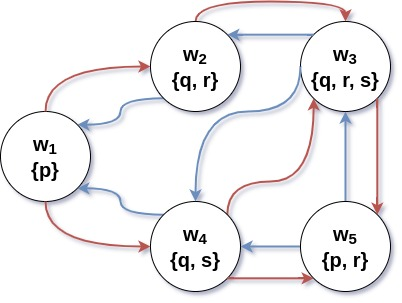
\includegraphics[width=0.5\linewidth]{images/example_3.jpg}
                    \centering
                    \caption{Reprezentare grafică a exemplului \ref{ex_modal_logic}}
                \end{figure}

                Analizând $\tau$-\textit{frame}-ul $\mathcal{F}=(W,\{R_1,R_2\})$ și $\tau$-modelul $\mathcal{M}=(\mathcal{F},L)$,
                se pot face următoarele observații:
                \begin{itemize}
                    \item Se verifică dacă $\mathcal{M},w_4 \Vdash \Box_1\Diamond_2 q$. Pentru a fi adevărată trebuie ca
                    orice stare x, accesibilă din $w_4$ prin relația $R_1$, să respecte $\mathcal{M},x \Vdash \Diamond_2 q$.
                    Deci, în stările $w_3$ și $w_5$ trebuie să fie adevărată formula $\Diamond_2 q$, ceea ce se întâmplă 
                    deoarece din starea $w_3$ este accesibilă starea $w_2$, prin relația $R_2$, în care este adevărată
                    formula q, iar din starea $w_5$ este accesibilă starea $w_3$, prin relația $R_2$. in care este 
                    adevărată formula q.
                    \item Se poate verifica afirmația $\mathcal{M} \Vdash \Box_1 (r \vee \Box_2 p)$. Este suficient să 
                    se arate că formula $r \vee \Box_2 p$ este adevărată pentru orice stare x accesibilă prin relația $R_1$
                    (pentru care există o stare y astfel încât $(y,x) \in R_1$). Aceste stări sunt $w_2$, $w_3$, $w_4$ și $w_5$.
                    Formula r este adevărată în toate aceste stări, mai puțin în $w_4$. Deci rămâne de arătat că 
                    $\mathcal{M},w_4 \Vdash \Box_2 p$, ceea ce este corect deoarece în starea $w_1$, unica accesibilă prin 
                    relația $R_2$ din $w_4$, formula p este adevărată în acest model.
                    \item Se poate demonstra că $\mathcal{F},w_1 \vDash \Box_1 \Diamond_1 p \rightarrow \Diamond_1 \Box_1 p$.
                    Se pleacă de la presupunerea că formula $\Box_1 \Diamond_1 p$ este validă în starea $w_1$, adică în 
                    stările $w_2$ și $w_4$, cele accesibile din $w_1$ prin relația $R_1$, trebuie ca formula $\Diamond_1 p$
                    să fie validă. Dar pentru starea $w_2$ există o singură stare accesibilă prin relația $R_1$, deci se
                    poate deduce și că formula $\Box_1 p$ este validă în starea $w_2$. Acest lucru implică faptul că, în starea $w_1$, 
                    este validă formula $\Diamond_1 \Box_1 p$, adică ceea ce se dorea.
                    \item Se poate arăta că $\mathcal{F} \vDash \varphi \rightarrow \Box_1 \Diamond_2 \varphi$. Această 
                    afirmație nu va fi demonstrată, ea fiind o consecință a unui caz mai general care va fi prezentat în
                    cele ce urmează.
                \end{itemize}
            \end{example}
            
            \par{}
                \noindent \textit{Observație:} Un \textit{frame} bidirecțional este un $\tau$-\textit{frame} ce conține 
                doar două relații binare de accesibilitate, $R_1$ și $R_2$, astfel încât una din relații este inversa 
                celelalte: $R_2=R_1^{-1}$ (pentru orice stări $x,y \in W$ se știe că $(x,y) \in R_1$ dacă și numai dacă 
                $(y,x) \in R_2$).
            
            \begin{sentence}
                Fie $\mathcal{F}=(W,\{R_1,R_2\})$ un $\tau$-\textit{frame}. $\mathcal{F}$ este un \textit{frame} 
                bidirecțional dacă și numai dacă afirmația $\mathcal{F} \vDash \varphi \rightarrow (\Box_1 \Diamond_2 
                \varphi \wedge \Box_2 \Diamond_1 \varphi)$ este adevărată pentru orice formulă $\varphi$.

                \begin{proof}[\textbf{Demonstrație:}]
                    Pentru început, se va demonstra implicația directă, adică se presupune că $\mathcal{F}$ este un 
                    \textit{frame} bidirecțional și se va arăta că $\mathcal{F} \vDash \varphi \rightarrow (\Box_1 
                    \Diamond_2 \varphi \wedge \Box_2 \Diamond_1 \varphi)$ pentru orice formulă $\varphi$. Se consideră o
                    formulă a logicii modale $\varphi$ și o stare $w \in W$ din \textit{frame}-ul $\mathcal{F}$ pentru 
                    care se știe că $\mathcal{F},w \vDash \varphi$. Pentru simplitate, se va demonstra doar validitatea 
                    uneia dintre cele două formule din conjuncție, cealaltă demonstrație fiind similară. În cele ce 
                    urmează se va arăta că $\mathcal{F},w \vDash \Box_1 \Diamond_2 \varphi$. Fie $y \in W$ o stare 
                    accesibilă din starea w prin relația $R_1$ ($(w,y) \in R_1$), se dorește ca $\mathcal{F},y \vDash 
                    \Diamond_2 \varphi$. Această ultimă afirmație este adevărată, deoarece $\mathcal{F},w \vDash 
                    \varphi$ și $(y,w) \in R_2$ (din bidirecționalitate și faptul că $(w,y) \in R_1$). Așadar, această 
                    implicație este adevărată.

                    Pentru implicația inversă, se știe că $\mathcal{F} \vDash \varphi \rightarrow (\Box_1 \Diamond_2 
                    \varphi \wedge \Box_2 \Diamond_1 \varphi)$ pentru orice formulă $\varphi$ și se urmărește să se arate 
                    că $\mathcal{F}$ este bidirecțional. Se presupune, prin reducere la absurd, că $\mathcal{F}$ nu este 
                    bidirecțional, deci rezultă că există două stări $x,y \in W$ pentru care $(x,y) \in R_1$ și $(y,x) 
                    \notin R_2$ sau $(x,y) \notin R_1$ și $(y,x) \in R_2$. Ținând cont de faptul că formula analizată 
                    este simetrică (dacă se interschimbă $\Box_1$ cu $\Box_2$ și $\Diamond_1$ cu $\Diamond_2$ se obține
                    aceeași formulă), se poate presupune, fără a restrânge generalitatea, că există două stări $x,y \in 
                    W$ pentru care $(x,y) \in R_1$ și $(y,x) \notin R_2$. Se va construi un $\tau$-model $\mathcal{M}=(
                    \mathcal{F},L)$, unde L este o funcție de evaluare, în care formula $p \rightarrow (\Box_1 
                    \Diamond_2 p \wedge \Box_2 \Diamond_1 p)$ nu este adevărată în starea x, astfel: $p \in L(x)$ și $p 
                    \notin L(w)$ pentru orice $w \in W$ cu $w \neq x$. Din această definiție se poate vedea ușor că 
                    formula p este adevărată în starea x ($\mathcal{M},x \Vdash p$). În plus, se știe că $(y,x) \notin 
                    R_2$ și $p \notin L(w)$ pentru orice $w \in W$ cu $w \neq x$, deci $\mathcal{M},y \nVdash \Diamond_2 
                    p$. Combinând acest rezultat cu faptul că $(x,y) \in R_1$, rezultă că $\mathcal{M},x \nVdash \Box_1 
                    \Diamond_2 p$. Recapitulând rezultate demonstrate, se cunoaște $\mathcal{M},x \Vdash p$ și 
                    $\mathcal{M},x \nVdash \Box_1 \Diamond_2 p$, deci este evident că nu se poate ca $\mathcal{M},x 
                    \Vdash p \rightarrow (\Box_1 \Diamond_2 p \wedge \Box_2 \Diamond_1 p)$, ceea ce contrazice presupunerea făcută. 
                    Deci \textit{frame}-ul considerat este bidirecțional.

                    Având în vedere că ambele sensuri ale implicație sunt adevărate, se poate afirma că propoziția 
                    analizată este adevărată.
                \end{proof}
            \end{sentence}

            \begin{example}
                O aplicație importantă a \textit{frame}-urilor bidirecționale este Limbajul Temporal De Bază 
                \myenglishterm{The Basic Temporal Language}. După cum a fost prezentat și în 
                \mysectionreference{section_engineering}, folosind logica modală se poate modela persistența unui adevăr
                în viitor. Acest model se dezvoltă, urmărindu-se și modelarea acțiunilor care s-au petrecut în trecut. 
                Concret, se pornește de la o similaritate de tip ce conține doi operatori unari, $O=\{[G], [H]\}$. 
                Aceștia sunt notați cu literele G și H, ce provin de la denumirea din limba engleză a expresiilor „va fi
                întotdeauna cazul” \myenglishterm{"it is always Going to be the case"} și „a fost întotdeauna cazul” 
                \myenglishterm{"it always Has been the case"} \cite{modal_logic}. Aceste expresii stau, de altfel, și la
                baza interpretării operatorilor, formula $[G]\varphi$ semnificând că „$\varphi$ va fi întotdeauna 
                adevărată” și formula $[H]\varphi$ că „$\varphi$ a fost întotdeauna adevărată”.

                În plus, se pot defini operatorii duali ai acestora, care se notează, de obicei, cu $<F>$ și $<P>$, de 
                la termenii din limba engleză viitor \myenglishterm{Future}, respectiv trecut \myenglishterm{Past}. 
                Folosindu-ne de modul în care sunt definiți acești operatori, se poate deduce și interpretarea acestora.
                Mai explicit, formula $<F> \varphi$ simbolizează că „$\varphi$ va fi adevărată la un moment dat în 
                viitor”, iar formula $<P> \varphi$ exprimă faptul că „$\varphi$ a fost adevărată la un moment dat în 
                trecut”. De multe ori, pentru o scriere mai curată a formulelor, operatori modali ($[G], [H], <F>, <P>$)
                sunt referențiați doar prin litera acestora, adică G, H, F, respectiv P.

                Este ușor de înțeles acum de ce este de dorit ca $\tau$-\textit{frame}-ul care stă la baza acestei 
                construcții să fie unul bidirecțional. Dacă aceasta nu ar fi adevărată, atunci ar fi posibil, de 
                exemplu, să existe un moment x în viitor raportat la un alt moment y, dar momentul y să nu existe în 
                trecut față de momentul x. Acest lucru nu are sens în problema care se dorește a fi modelată și, în 
                plus, conduce la invalidarea multor altor adevăruri. De exemplu, formula $P \varphi \rightarrow G P 
                \varphi$, care se interpretează ca „Dacă $\varphi$ a fost adevărată la un moment dat, atunci va fi 
                întotdeauna adevărat că $\varphi$ a fost adevărată la un moment din trecut”, nu ar rămâne validă într-un 
                $\tau$-\textit{frame} care nu are proprietatea de bidirecționalitate. Formula anterior menționată 
                ilustrează proprietatea de non-repudiere a unui eveniment (odată petrecut un eveniment, existența 
                acestuia nu mai poate fi negată).

                O cerință interesantă, care nu poate fi satisfăcută folosind limbajul temporal de bază, este modelarea 
                expresiilor „din acel moment” \myenglishterm{since} și „până la acel moment” \myenglishterm{until}. O 
                soluție pentru aceasta este oferită de logica hibridă, care adaugă limbajului modal posibilitatea de a 
                referi în cadrul unei formule o lume din contextul \textit{frame}-ul \cite{handbook_modal_logic}.
            \end{example}

            \begin{example}
                Un alt caz din logica modală care merită menționat este cel prin care a fost motivată necesitatea utilizării 
                mai multor operatori modali, și anume modelarea cunoștințelor mai multor agenți. Se consideră problema 
                reprezentării pentru un număr finit de n agenți pentru care se definește mulțimea $O=\{\Box_1, \Box_2, 
                ..., \Box_n\}$. Similar cu problema unui singur agent, discutată în 
                \mysectionreference{section_engineering}, formula $\Box_i \varphi$ se interpretează ca fiind „Agentul i 
                știe $\varphi$”. Avantajul acestui nou model este că se pot reprezenta interacțiunile dintre agenți. 
                De exemplu, se poate afirma că formula $\Box_i (p \wedge \Box_j q)$ este adevărată, adică „Agentul i 
                cunoaște afirmația p, dar știe și că agentul j cunoaște informația q”.
            \end{example}

            \begin{example}
            \label{ex_pdl}
                Ultimul exemplu abordat în această secțiune este și cel care ilustrează cel mai bine puterea de modelare
                conferită de limbajul logicii modale. Acesta este reprezentat de Logica Propozițională Dinamică 
                \myenglishterm{Propositional Dynamic Logic}. Acest limbaj este foarte interesant atât din punct de 
                vedere practic, întrucât ajută la modelarea execuției programelor, cât și dintr-un punct de vedere 
                teoretic, deoarece se bazează pe o similaritate modală ce conține un număr infinit de operatori modali. 
                Mai precis, operatori din mulțimea O au forma $[\pi]$, unde $\pi$ reprezintă un program care poate fi și 
                nedeterminist, iar operatorul dual este $<\pi>$. Interpretarea formulei $[\pi] \varphi$ este că „după 
                terminarea oricărei execuții a programului $\pi$ este adevărată proprietatea $\varphi$, iar a formulei 
                $<\pi> \varphi$ este că „există o execuție a programului $\pi$ la sfârșitul căreia este adevărată 
                proprietatea $\varphi$”.

                Așa cum a fost prezentat anterior, definirea operatorilor modali din acest limbaj este dată de mulțimea 
                programelor analizate. Așadar, pentru a defini complet signatura modală a limbajului, trebuie să fie 
                descrisă mai întâi mulțimea programelor, acest lucru fiind realizat inductiv. Similar cu propozițiile logicii,
                se definește o mulțime de programe atomice pe care se pot aplica secvențial mai mulți operatori 
                specifici pentru a se obține alte programe. Regulile folosite pentru crearea noilor programe sunt 
                asemănătoare cu regulile folosite pentru definirea expresiilor regulate și pot fi descrise astfel 
                \cite{dynamic_logic}:
                \begin{itemize}
                    \item [] \textbf{compunere \myenglishterm{composition}}: Dacă $\pi_1$ și $\pi_2$ sunt programe, 
                    atunci și $(\pi_1; \pi_2)$ este program. Semnificația acestuia este „Execută secvențial programul 
                    $\pi_1$ și apoi programul $\pi_2$”. 
                    \item [] \textbf{alegere \myenglishterm{choice}}: Dacă $\pi_1$ și $\pi_2$ sunt programe, 
                    atunci și $(\pi_1 \cup \pi_2)$ este program. Semnificația acestuia este „Alege nedeterminist unul 
                    din programele $\pi_1$ sau $\pi_2$ și execută-l”. 
                    \item [] \textbf{iterație \myenglishterm{iteration}}: Dacă $\pi$ este un program, atunci și 
                    $(\pi^\star)$ este program. Semnificația acestuia este „Se execută programul $\pi$ de un număr finit 
                    de ori ales în mod nedeterminist”.
                    \item [] \textbf{testare \myenglishterm{test}}: Dacă $\varphi$ este o formulă, atunci $(\varphi?)$ 
                    este un program. Semnificația acestuia este „Testează formula $\varphi$, dacă este adevărată 
                    continuă, altfel execuția se oprește”.
                \end{itemize}

                Cu ajutorul acestor operatori se pot descrie formule mai complexe, cum ar fi formula $<\pi^\star>\varphi 
                \leftrightarrow \varphi \vee <\pi; \pi^\star>\varphi$ exprimă că o stare în care $\varphi$ este adevărată
                poate fi atinsă executând programul $\pi$ de un număr finit de ori dacă și numai dacă $\varphi$ este 
                adevărată în starea curentă sau dacă executând programul $\pi$ cel puțin o dată se ajunge într-o stare 
                în care $\varphi$ este adevărată. O altă formulă importantă pentru limbajul propozițional dinamic este
                $\varphi \rightarrow ([\pi^\star](\varphi \rightarrow [\pi]\varphi) \rightarrow [\pi^\star]\varphi)$, 
                cunoscută și sub denumirea de axioma lui Segerberg \cite{lecture_notes_hedin}. Chiar dacă nu pare 
                evident, aceasta ilustrează un principiu matematic bine cunoscut, principiul inducției. O explicație 
                pentru aceasta poate fi dată de interpretarea formulei: „Dacă se cunoaște $\varphi$ (pasul inițial, 
                P(0)) și, în plus, se știe că, după un număr aleator finit de execuții ale programului $\pi$, dacă 
                formula $\varphi$ este adevărată atunci aceasta va fi adevărată și după încă o execuție a programului 
                $\pi$ (pasul inducției, P(n) $\Rightarrow$ P(n+1)), atunci se poate deduce că $\varphi$ este 
                adevărată după un număr arbitrar finit de execuții ale programului $\pi$(concluzia inducției, P(n) 
                adevărată pentru orice n)”. Această axiomă are o importanță deosebită în verificarea corectitudinii 
                secvențelor de cod repetitive, precum „for” sau „while”, aceste verificări putând fi rezumate, de 
                multe ori, la demonstrarea conservării unor proprietății de la o iterație la alta.

                Un alt lucru important care nu a fost încă prezentat este legat de relațile de accesibilitate. Se știe 
                că pentru fiecare operator dintr-un sistem al logicii modale trebuie să se definească o relație de 
                accesibilitate. Aceasta poate deveni o problemă dificilă sau chiar una imposibil de rezolvat în 
                contextul unui model care conține un număr infinit de operatori. În ceea ce privește modelarea limbajului 
                propozițional dinamic, acest fapt nu reprezintă o dificultate deoarece fiecare regulă de construcție a 
                programelor definește o regulă pentru relația de accesibilitate a programului nou format. Deci,
                ținând cont de aceasta, este suficient să se definească relațiile de accesibilitate doar pentru mulțimea 
                de programe atomice, adică o mulțime finită. Reguli ce pot fi folosite pentru definirea relațiilor de 
                accesibilitate sunt următoarele \cite{lecture_notes_hedin}:
                \begin{align*}
                    R_{\pi_1 \cup \pi_2} &= R_{\pi_1} \cup R_{\pi_2} \\
                    R_{\pi_1; \pi_2} &= R_{\pi_1} \circ R_{\pi_2} \; (= \{(x,y) | \exists z ((x,z) \in R_{\pi_1} \wedge (z,y) \in R_{\pi_2}) \})\\
                    R_{\pi^\star} &= (R_{\pi})^\star \; (= \{(x,y) | \exists k \in \mathbb{N} ((x,y) \in R_{\pi}^k) \})
                \end{align*}
            \end{example}

            \par{}
                \noindent \textit{Observație}: Un \textit{frame} construit pe baza regulilor prezentate în exemplul 
                anterior poartă denumirea de \textit{frame} normal \myenglishterm{regular frame}. 
                
            \begin{sentence}
                Fie $\mathcal{F}=(W,\{R_\pi | \pi \in \Pi\})$ ($\Pi$ reprezintă mulțimea programelor) un 
                \textit{frame}. $\mathcal{F}$ este un \textit{frame} normal dacă și numai dacă $\mathcal{F} \vDash 
                \Delta \cup \Gamma$, unde:
                \begin{align*}
                    \Delta := &\{p \rightarrow ([\pi^\star](p \rightarrow [\pi]p) \rightarrow [\pi^\star]p) | \pi \in \Pi \} \cup \\
                              & \{<\pi^\star>p \leftrightarrow p \vee <\pi><\pi^\star>p | \pi \in \Pi \} \\
                    \Gamma := &\{<\pi_1; \pi_2> p \leftrightarrow <\pi_1><\pi_2>p | \pi_1,\pi_2 \in \Pi \} \cup \\
                              & \{<\pi_1 \cup \pi_2>p \leftrightarrow <\pi_1>p \vee <\pi_2>p | \pi_1,\pi_2 \in \Pi \}
                \end{align*}
            \end{sentence}

            \par{}
                Acest rezultat de caracterizare a \textit{frame}-urilor regulate este foarte important pentru limbajul 
                propozițional dinamic deoarece oferă totodată și bazele unui sistem în care se pot demonstra proprietăți 
                ale programelor. Concret, acest sistem poate fi creat folosind o structură similară cu exemplele 
                prezentate în \mysectionreference{section_normal_modal_logics}, formulele ce caracterizează 
                \textit{frame}-urile regulate putând fi folosite ca axiome ale unui astfel de sistem.
        % section Generalizarea  logicii modale de bază (end)
    % chapter Logică Modală (end)

    \chapter{Verificator de demonstrații} % (fold)
    \label{chapter_demonstration_checker}

        \section{Prezentarea problemei} % (fold)
        \label{section_intro_checker}
            \par{}
                Scopul acestui capitol este de a prezenta un exemplu practic pentru a ilustra cum pot fi folosite conceptele 
                teoretice din logica modală pentru rezolvarea unor probleme concrete. După cum a fost prezentat în 
                \mysectionreference{chapter_modal_logic}, logica modală poate ajuta la modelarea diverselor probleme și la
                demonstrarea anumitor proprietăți, însă nu s-a făcut nici o referire la modul în care pot fi automatizate 
                aceste procese. Acesta reprezintă subiectul ce va fi abordat în continuare, accentul fiind pus pe 
                construirea unui verificator de demonstrații.

            \par{}
                În majoritatea problemelor, se dorește determinarea proprietăților care sunt valabile într-un caz 
                general, nu doar într-un context particular. În terminologia folosită în logică, acest lucru s-ar 
                traduce prin noțiunea de validitate a formulelor, iar un instrument puternic pentru testarea validității
                este reprezentat de demonstrațiile sintactice. Acestea sunt prezente în multe sisteme logice, nefiind 
                specifice numai logicii modale. O problemă semnificativă în cazul acestor demonstrații este că, deși 
                regulile ce le definesc sunt complete și corecte, din cauza complexității pe care le ating, pot apărea 
                erori umane de-a lungul realizării lor. În acest context, au apărut verificatoarele de demonstrații 
                automate, care pot avea implementate regulile de deducție ale sistemului pe care le folosesc pentru a 
                verifica dacă demonstrația realizată este corectă, eliminând astfel complet erorile apărute pe parcurs. 
                Restrângând această problemă la contextul logicii modale, un verificator de demonstrații poate fi 
                utilizat în verificarea corectitudinii \textbf{K}-demonstrațiilor, concept prezentat pe larg în 
                \mysectionreference{section_normal_modal_logics}. 
                
            \par{}
                Construirea unui astfel de verificator pentru logica modală reprezintă obiectul acestui capitol. 
                Concret, va fi prezentat un modul propriu, denumit \textbf{ModalProofChecker}, realizat folosind limbajul Haskell. 
                Acesta modelează conceptele necesare pentru realizarea 
                \textbf{K}-demonstrațiilor și oferă o funcționalitate ce permite verificarea acestor demonstrații. În 
                cele ce urmează, vor fi prezentate atât detaliile legate de implementarea acestui modul, precum noile 
                tipuri de date definitie și cele mai importante funcții utilizate în verificarea demonstrațiilor, cât și 
                mențiuni utile pentru utilizarea acestuia cum ar fi formatul în care trebuie să fie scrise 
                demonstrațiile și cum pot fi verificate acestea. Este important de menționat faptul că acest exemplu se 
                rezumă la limbajul modal de bază, deci oferă posibilitatea utilizării doar a unei perechi de operatori
                modali, $\Box$ și $\Diamond$.
        % section Prezentarea problemei % (end)

        \section{Alegerea limbajului de programare} % (fold)
        \label{section_haskell}
            \par{}
                Înainte de a intra în detalii specifice implementării exemplului, este oferită o justificare pentru 
                alegerea limbajului de programare Haskell în dezvoltarea acestui verificator de demonstrații. Motivația acestei 
                secțiuni nu este de a explica de ce trebuie să fie utilizat Haskell pentru acest exemplu, având în vedere că implementarea acestei probleme 
                putea fi realizată în multe alte limbaje de programare, ci de a prezenta avantajele utilizării acestui limbaj, în acest caz concret. 
                
            \par{}
                Un punct cheie pentru implementarea unui 
                verificator de demonstrații, sau a unui sistem logic în general, este reprezentat de capacitatea de a 
                modela conceptele logice abstracte. Din acest punct de vedere, Haskell a oferit un avantaj considerabil,
                poate în acest caz particular mai mare decât un limbaj orientat pe obiecte 
                \myenglishterm{object oriented}, fiind un limbaj cunoscut pentru puterea sa de modelare 
                \cite{haskell_documentation}. O altă caracteristică a limbajului, care îmbunătățește procesul de 
                implementare, este constituită de utilizarea funcțiilor șablon \myenglishterm{pattern 
                matching}. Acest aspect poate fi neînsemnat în unele cazuri, dar în altele, precum cel de față în care 
                este întâlnită des inducția pe formule, are un rol foarte important în separarea fiecărui caz. În afară, 
                de acestea, se mai pot menționa și alte avantaje ale limbajului Haskell, precum codul compact sau 
                puritatea funcțiilor.
        % section Alegerea limbajului de programare % (end)

        \section{Modelarea conceptelor} % (fold)
        \label{section_data_type}
            \par{}
                Pentru început, va fi făcută o prezentare a modului în care au fost modelate conceptele logice necesare 
                pentru a rezolva problema. Dintre acestea, vor fi prezentate formulele, regulile de deducție, sistemul 
                de deducție și demonstrațiile.

            \begin{lstlisting}
                data Proof = Proof Deduction_System [(Formula, Deduction_Rule)]
                             deriving Show
            \end{lstlisting}

            \par{}
                Primul tip de dată considerat este cel care le înglobează pe toate celelate, \texttt{Proof}. Acesta 
                modelează noțiunea de demonstrație pentru care sunt necesare un \texttt{Deduction\_System}, contextul în 
                care este realizată demonstrația, și o listă a căror elemente sunt perechi de \texttt{Formula} și 
                \texttt{Deduction\_Rule}, fiecare dintre acestea reprezentând formula dedusă și regula utilizată pentru 
                deducția acesteia. Ordinea în care sunt deduse formulele de-a lungul demonstrației este importantă în 
                sensul în care, pentru demonstrarea formulei de pe poziția i, nu pot fi folosite formulele de pe 
                pozițiile i+1, i+2 și așa mai departe. În cadrul demonstrațiilor, aceste poziții vor fi folosite pentru 
                a identifica formulele deja deduse. De exemplu, dacă se dorește utilizarea regulii „modus ponens”, 
                pentru a specifica pe ce formule se aplică, vor fi utilizate aceste numere de ordine. Indexarea 
                formulelor începe de la 1, această decizie fiind luată deoarece în demonstrațiile logice acest lucru 
                este mult mai des întâlnit decât indexarea de la 0. În continuare, vor fi detaliate tipurile 
                de date care compun \texttt{Proof}.

            \begin{lstlisting}
                type Atom = String

                data Formula = F | T
                               | AtomF Atom
                               | NotF Formula 
                               | AndF Formula Formula
                               | OrF Formula Formula
                               | ImpF Formula Formula
                               | EqvF Formula Formula
                               | BoxF Formula
                               | DiaF Formula
                               | ErrorF
                               deriving Eq
                infixl 7 `AndF`
                infixl 6 `OrF`
                infixr 5 `ImpF`
                infixr 5 `EqvF`
            \end{lstlisting}

            \par{}
                Discuția va continua cu modelarea formulelor din limbajul modal de bază. Definiția tipului de date 
                \texttt{Formula} reprezintă o transpunere în limbajul Haskell a definiției \ref{def_basic_synthax}. 
                Pentru reprezentarea formulelor ce semnifică adevărul ($\top$) și falsul ($\bot$) sunt utilizați 
                constructori fără parametrii \texttt{T}, respectiv \texttt{F}. Pentru atomi propoziționali, cei din 
                mulțimea $Prop$, este utilizat constructorul de date \texttt{AtomF} împreună cu denumirea atomului. Se 
                observă faptul că denumirea atomilor este de tip \texttt{Atom}, care nu este decât o altă denumire 
                pentru tipul \texttt{String}, utilizată pentru claritatea modelării. În plus, utilizarea tipului 
                \texttt{String} ca tip de bază al denumiri atomilor permite folosirea unei mulțimi arbitar de mare de 
                atomi propoziționali. În ceea ce privește ceilalți constructori din definiția tipului de date 
                \texttt{Formula}, aceștia modelează operatori logici conform următoarelor corespondențe: \texttt{NotF} 
                și $\neg$, \texttt{AndF} și $\wedge$, \texttt{OrF} și $\vee$, \texttt{ImpF} și $\rightarrow$, 
                \texttt{EqvF} și $\leftrightarrow$, \texttt{BoxF} și $\Box$, \texttt{DiaF} și $\Diamond$. Ultimul caz, 
                cel al constructorului \texttt{ErrorF}, este folosit pentru a semnala diverse erori care pot apărea în 
                funcțiile care întorc date de tipul \texttt{Formula}. Aceste cazuri speciale vor fi detaliate în 
                descrierea funcțiilor care folosesc acest constructor. De asemenea, se pot observa utilizarea funcțiilor 
                \texttt{infixr} și \texttt{infixl} care permit stabilirea de priorități pentru constructorii de date 
                binari. Aceasta are o consecință foarte importantă, permițând scrierea mult mai clară a formulelor, 
                deoarece sunt eliminate multe paranteze. Numărul întreg din apelul funcțiilor reprezintă prioritatea 
                asociată fiecărui operator, putându-se observa faptul că \texttt{AndF} are cea mai mare prioritate, apoi 
                evaluându-se constructorul \texttt{OrF} și, în final, \texttt{ImpF} și \texttt{EqvF}. Important de 
                menționat este că pentru a beneficia de această facilitate trebuie să fie folosită forma infixată a 
                constructorilor (plasarea între operanzi) și nu forma prefixată a acestora (plasarea înaintea 
                operanziilor).

            \begin{lstlisting}
                newtype Deduction_System = Axioms { get_axioms :: [Formula]}
                                           deriving Show
            \end{lstlisting}

            \par{}
                Tipul de date \texttt{Deduction\_System} este utilizat pentru a încapsula contextul în care este 
                realizată demonstrația. Concret, în cazul acesta, demonstrația este influențată de formulele ce sunt 
                considerate axiome. De menționat este și faptul că, similar formulelor deduse, și axiomelor li se 
                asociază un număr de ordine pentru a putea fi utilizate în cadrul demonstrațiilor. De asemenea, la fel 
                ca în cazul formulelor, și această indexare se realizează începând de la 1. Se poate observa că definirea 
                tipului de date folosind această scriere conduce și la crearea unei funcții „getter” pentru lista de axiome, numită 
                \texttt{get\_axioms}.

            \begin{lstlisting}
                data Deduction_Rule = Axiom Int
                                    | Taut
                                    | KAxiom
                                    | DualAxiom
                                    | MP Int Int
                                    | US Int
                                    | Gen Int
                                    deriving Show
            \end{lstlisting}

            \par{}
                Următorul tip de dată prezentat este \texttt{Deduction\_Rule}, care modelează conceptul de regulă de 
                deducție. Conceptul este extins față de definiția regulilor de deducție din capitolul anterior, în 
                sensul în care sunt adăugate și câteva reguli care semnifică deducția axiomelor (\texttt{Axiom}, 
                \texttt{Taut}, \texttt{KAxiom} și \texttt{DualAxiom}). Constructorul \texttt{Axiom} modelează deducerea 
                formulelor ce sunt instanțe ale unei axiome a sistemului, numărul asociat reprezintând numărul de ordine 
                al axiomei utilizate. Următoarele trei cazuri, \texttt{Taut}, \texttt{KAxiom} și \texttt{DualAxiom}, 
                modelează tot deducții ale axiomelor și anume al instanțelor tautologiilor din logica propozițională, al 
                axiomei K, respectiv al axiomei duale. Este important ca pentru deducția instanțelor acestor axiome să 
                existe o regulă diferită față de cea a deducerii unei axiome adăugate în sistemul de deducție, deoarece 
                orice sistem de deducție considerat trebuie să conțină axiomele K, duală și toate tautologiile din 
                logica propozițională. Ultimii trei constructori se referă la cazurile de deducție din sistemul logicii 
                modale „modus ponens”, substituția uniformă și respectiv generalizarea. Parametrii pe care aceștia îi 
                primesc reprezintă numerele de ordine, din cadrul demonstrației, ale formulelor folosite în aplicarea 
                acestor reguli.

            \par{}
                Acestea reprezintă cele mai importante tipuri de date utilizate în construirea verificatorului de 
                demonstrații. Odată cu introducerea formatului unei demonstrații, poate fi descrisă abordarea utilizată 
                în implementarea verificatorului. Concret, trebuie realizată o funcție care testează corectitudinea unei 
                demonstrații încapsulate într-o dată de tipul \texttt{Proof}. Pentru aceasta, va trebui să se verifice 
                modul în care a fost dedusă fiecare formulă de-a lungul demonstrație.
        % section Modelarea conceptelor (end)

        \section{Descrierea funcționalității} % (fold)
        \label{section_functionality}
            \par{}
                În această secțiune, vor fi prezentate detaliile implementării modulului \textbf{ModalProofChecker}. 
                Înainte de a prezenta funcțiile, trebuie introduse câteve tipare utilizate mai frecvent în funcțiile 
                acestui modul. Pentru a putea avea un cod flexibil și mentenabil, procesul de testare a demonstrațiilor 
                a fost împărțit în unități mai mici, fiecare dintre acestea fiind rezolvată de o funcție diferită. Pe de 
                altă parte, această abordare conduce la alte provocări. De exemplu pentru returnarea motivului unei 
                erori apar dificultăți deoarece, chiar dacă este depistată cauza, aceasta trebuie să fie trimisă prin 
                mai multe funcții, până când ajunge la utilizator. Pentru rezolvarea acestei probleme, va fi utilizată 
                monada \texttt{Writer} care permite menținerea atât a unei valori, cât și a altor informații utile. În 
                cazul de față, este utilizată monada \texttt{Writer [String] Bool}, informația reținută fiind 
                reprezentată de o listă de mesaje care, în cazul unei erori, semnifică motivele acesteia, de la cel mai 
                specific la cel mai general, asemănător unui \textit{stack trace}. Mai multe exemple care ilustrează 
                aceste cazuri pot fi găsite în \mysectionreference{section_usage}. 
                
            \par{}
                O altă tehnică des utilizată în scrierea funcțiilor din modul este cea a inducției pe formule. Pentru a 
                fi mai explicit, este vorba despre cazul funcțiilor care trebuie să efectueze un calcul pentru o formulă 
                dată. Soluția presupune împărțirea acestei probleme în mai multe subprobleme în funcție de operatorul 
                „principal” al formulei, apoi definindu-se modul în care trebuie efectuat calculul dorit pentru fiecare 
                caz. Prin operator principal se înțelege operatorul ce are prioritatea cea mai mică (este interpretat 
                ultimul) din cadrul formulei.

            \par{}
                Acestea fiind spuse, în cele ce urmează va fi prezentată funcția principală a acestui modul, și anume 
                \texttt{verify\_proof}, ce reprezintă principalul punct de interacțiune al utilizatorilor cu modulul. 
                Această funcție primește ca argument o demonstrație de tipul \texttt{Proof}, după care apelează funcția 
                \texttt{verify\_proof\_recursive}. Asupra răspunsului primit de la această funcție, care este de tipul 
                monadei \texttt{Writer}, este aplicată funcția \texttt{runWriter} pentru a extrage rezultatul 
                verificării, precum și mesajele de eroare, dacă este cazul. Acestea sunt returnate către utilizator cu 
                mențiunea că lista mesajelor de eroare este inversată, deoarece se dorește ca acestea să fie ordonate de 
                la cel mai generic la cel mai specific. 
            
            \par{}
                După cum se poate observa și din denumirea funcții \texttt{verify\_proof\_recursive}, pentru realizarea 
                verificării demonstrației se va folosi o metodă recursivă. Mai precis, pentru testarea corectitudinii 
                unei demonstrații în care sunt deduse $n$ formule, trebuie să fie testată demonstrația formată din 
                primele $n-1$ deducții (\texttt{are\_previous\_deductions\_correct}) și corectitudinea ultimei deducții 
                (\texttt{is\_current\_deduction\_correct}). Dacă toate verificările sunt efectuate cu succes atunci 
                demonstrația este evaluată ca fiind corectă, altfel programul va întoarce o eroare, iar la lista
                mesajelor va fi adăugat faptul că deducția curentă este greșită (\texttt{wrong\_deduction\_message \$ 
                length fs}). Este important că, deoarece apelul recursiv este realizat înaintea verificării deducției 
                curente, dacă există mai multe greșeli de-a lungul demonstrației atunci va fi detectată și semnalată 
                prima dintre ele. Pasul de oprire al recursivității este dat în prima descriere a funcției (pentru 
                cazul în care demonstrația nu are nici o deducție, atunci demonstrația este considerată corectă). Pentru 
                verificarea corectitudinii unei deducții se poate observa că este utilizată funcția 
                \texttt{verify\_deduction}, care va fi prezentată în cele ce urmează.

            \par{}
                Scopul funcției \texttt{verify\_deduction} este de a verifica dacă o deducție este corectă. Înainte de a 
                intra în detalii pentru fiecare caz considerat, va fi discutată signatura funcției. Primul argument este 
                o listă a axiomelor sistemului în care se lucrează. În afară de aceste axiome, este necesar să se 
                cunoască și formulele care au fost deduse înainte de pasul curent, deoarece și acestea pot fi utilizate 
                în deducerea formulei curente. De aceea, al doilea parametru reprezintă o listă a formulelor care au 
                fost deduse până în acest moment, fără regulile folosite pentru deducția acestora, deoarece nu sunt 
                necesare. Următoarele două argumente semnifică formula analizată la acest pas, precum și regula de 
                deducție utilizată pentru obținerea ei. 
            
            \par{}
                La acest pas, sunt efectuate mai multe verificări pentru indicii axiomelor și inidicii formulelor asupra 
                cărora sunt aplicate regulile de deducție. Dacă una dintre aceste testări eșuează, atunci demonstrația 
                este greșită și, ca atare, va fi adăugat un mesaj sugestiv pentru eroarea detectată. Mai precis, indicii 
                axiomelor trebuie să fie numere întregi mai mari ca 0 (\texttt{reason\_index\_ axiom\_too\_small}), dar 
                să fie și cel mult egali cu numărul de axiome din sistemul în care este realizată demonstrația 
                (\texttt{reason\_index\_axiom\_too\_big}). În cazul indicilor formulelor, după cum a fost menționat și 
                anterior, trebuie ca acestea să fie de asemenea numere întregi strict pozitive 
                (\texttt{reason\_index\_formula\_too\_small}) și mai mici decât indicele axiomei curente 
                (\texttt{reason\_index \_formula\_too\_big}). De asemenea, se poate observa că și în cazul regulii „modus 
                ponens” (\texttt{reason \_wrong\_modus\_ponens}) și al generealizării 
                (\texttt{reason\_wrong\_generalisation}) sunt adăugate mesaje de eroare, în caz de eșec. Celelalte 
                cazuri sunt mai complexe și pot conduce la apariția unor greșeli mai diverse. Ca urmare, tratarea 
                acestora este realizată în funcțiile mai specifice.
            
            \par{}
                Pe lângă acestea, funcția \texttt{verify\_deduction} ajută la separarea verificării regulilor de 
                deducție. Practic, fiecare regulă este testată independent de o funcție diferită, iar aceasta îmbină 
                rezultatele tuturor. Spre exemplu, în primul caz din această definiție este apelată funcția 
                \texttt{verify\_axiom} pentru a verifica dacă formula dată a fost dedusă îm mod corect ca fiind instanță 
                a axiomei referite prin indicele specificat. Este de remarcat că funcția \texttt{verify\_axiom} este 
                utilizată și pentru cazul instanțelor axiomei K, axiomei duale, folosindu-se argumente diferite. În timp 
                ce pentru cazul axiomelor menționate în cadrul sistemului de deducție sunt utilizate formulele extrase 
                din lista de axiome, pentru cazul axiomei K se utilizează variabila \texttt{axiom\_k}. Pentru celelate 
                cazuri rămase sunt verificate regulile astfel: \texttt{verify\_tautology} pentru tautologii, 
                \texttt{verify\_mp} pentru „modus ponens”, \texttt{verify\_usubs} pentru substituția uniformă și 
                \texttt{verify\_gen} pentru regula generalizării.
            
            \par{}
                Alt lucru care trebuie menționat este că această funcție realizează o transformare de la un mod de 
                indexare la altul (\texttt{ind\_axiom-1} sau \texttt{ind\_form-1}). Mai precis, este vorba de trecerea 
                de la numerotarea axiomelor din sistemul deductiv și a formulelor deduse de-a lungul demonstrației (care 
                se realizează începând de la 1) la indexarea listelor din Haskell (care se realizează începând de la 0). 
                În cele ce urmează, a rămas de prezentat doar implementarea pentru funcțiile care verifică fiecare 
                regulă de deducție.

            \par{}
                Prima funcție dintre cele care verifică regulile de deducție este \texttt{verify\_axiom}. Aceasta 
                primește ca prim argument o axiomă, iar al doilea argument este formula dedusă la pasul curent. Scopul 
                funcției este să returneze dacă formula dată este o instanță a axiomei primite ca parametru. Soluția 
                pentru aceasta este foarte simplă. Se va utiliza funcția \texttt{verify\_usubs}, ce va fi detaliată 
                ulterior. Folosind această funcție se poate verifica dacă formula dorită poate fi obținută din axioma 
                dată printr-o substituție uniformă. În caz afirmativ, rezultând faptul că într-adevăr este o instanță a 
                acesteia, altfel deducția făcută este greșită ca urmare va fi adăugat un mesaj corespunzător 
                (\texttt{reason\_no\_instance\_axiom}).

            \par{}
                În privința funcției ce se ocupă de verificarea tautologiilor \texttt{verify\_tautology}, abordarea este 
                puțin mai complexă, testarea putând fi împărțită în două componente distincte. În prima etapă, se 
                determină toți atomi propoziționali din formulă, pentru ca după să se poată obține toate evaluările 
                posibile. Apoi, în cea de a doua parte formula va fi evaluată folosind toate evaluările găsite în prima 
                parte. Înainte acestor pași este verificat faptul că formula dată nu conține operatori modali, deci este 
                o formulă din logica propozițională. În caz contrar, se adaugă un mesaj care să descrie eroarea produsă 
                (\texttt{reason\_modal\_operator\_in\_tautology}). Constructorul \texttt{LabelFunc} este folosit pentru 
                definirea unui tip de date ce modelează funcția de evaluarea din logica propozițională. Scopul 
                utilizării acestui tip de date este de a putea afișa funcțiile de evaluare folosind clasa \texttt{Show}.

            \par{}
                Funcția \texttt{get\_atoms} primește ca parametru o formulă și trebuie să întoarcă o listă cu 
                denumirile atomilor propoziționali ce se regăsesc în formula dată. Funcția are o structură specifică 
                unei operații bazate pe inducția pe formule, fiind descrise reguli pentru fiecare operator. Mai precis, 
                formulele $F$ și $T$ nu au nici un atom în compoziția lor, iar în cazul formulelor formate doar dintr-un 
                atom propozițional, lista atomilor îl conține doar pe acesta. În cazul operatorilor unari este suficient 
                să se determine lista atomilor din formula obținută prin eliminarea operatorului, iar pentru operatori 
                binari trebuie să se facă reuniunea listelor de atomi obținute din fiecare operand. Este de menționat și 
                faptul că pentru ca rezultatul funcției să fie o mulțime de atomi, trebuie utilizată funcția
                \texttt{nub} pentru eliminarea duplicatelor. Funcția \texttt{get\_evaluations} este utilizată pentru a 
                genera toate evaluările posibile pentru o mulțime de atomi. O funcție de evaluare este reprezentată ca o 
                listă de perechi de atomi propoziționali cu valoarea lor de adevăr. Aceste evaluări vor fi utilizate mai 
                departe pentru a determina dacă formula evaluată este sau nu tautologie.

            \par{}
                Pentru a încheia discuția despre verificarea tautologiilor, trebuie să se analizeze și partea de 
                evaluare a formulelor. Funcția \texttt{truth\_table} modelează conceptul de tabel de adevăr, primind ca 
                prim parametru mai multe funcții de evaluare în formatul descris anterior, iar al doilea argument este o 
                formulă. Este evaluată formula primită ca argument folosind toate funcțiile de evaluare date. 
                Verificarea este oprită imediat ce este găsită o funcție de evaluare pentru care formulă este falsă, 
                întrucât în acest caz formula considerată nu poate fi tautologie. În plus, mesajul returnat ce 
                explicitează eroare va conține și funcția de evaluarea ce invalidează proprietatea de tautologie a 
                formulei (\texttt{reason\_no\_tautology eval}). Pentru interpretarea efectivă a formulelor este 
                utilizată funcția \texttt{evaluation}, care primește ca parametri o funcție de evaluare și o formulă. 
                Similar cu funcția \texttt{get\_atoms}, și această funcție se bazează pe inducția pe formule, regulile 
                pentru fiecare caz fiind descrise de definiția funcțiilor de evaluare din logica propozițională.
            
            \par{}
                Până acum au fost descrise funcțiile pentru verificarea regulilor care se refereau la deducția 
                axiomelor. În continuare, rămâne de prezentat modul în care sunt verificate și 
                regulile de deducție clasice, cele definite și în sistemul \textbf{K}. Dintre acestea, se va face 
                referire pentru început la cea mai cunoscută dintre ele, și anume „modus ponens”. 

            \par{}
                Funcția \texttt{verify\_mp} primește ca argumente trei formule, primele două dintre ele fiind cele 
                asupra căreia este aplicată regula, iar ceea de-a treia reprezentând rezultatul obținut. Pentru 
                verificarea corectitudinii acestei reguli trebuie verificate următoarele: (1) una din primele două 
                formule să fie o implicație, (2) premisa acelei implicații să fie cealaltă formulă dintre primele două 
                și (3) ultima formulă să fie concluzia implicației. Doar dacă cele trei afirmații sunt toate adevărate 
                regula este adevărată, în orice alt caz regula fiind aplicată greșit.

            \par{}
                Următoare regulă de deducție ce va fi abordată este generalizarea. Această regulă spune că dacă o 
                formulă $\varphi$ este validă, atunci și formula $\Box \varphi$ este validă. Deci în funcția 
                \texttt{verify\_gen} care se ocupă de verificarea aplicării acesteia, trebuie testat dacă formula 
                dedusă (al doilea argument) este generalizarea formulei pe care s-a aplicat regula (primul argument).

            \par{}
                Ultima regulă rămasă este substituția uniformă, a cărei verificare este realizată de către funcția 
                \texttt{verify\_usubs}. Abordarea în cazul acestei reguli de deducție este mai complexă decât în 
                celelalte două cazuri, aceasta deoarece în cazul substituției uniforme trebuie să se determine o funcție
                de substituție care să facă transformarea de la o formulă la alta. Mai concret, funcția
                \texttt{verify\_usubs} primește ca argument două formule, cea pe care s-a aplicat regula și cea care a 
                fost obținută, iar testarea regulii se împarte în două etape obținerea unei funcții de substituție și 
                verificarea corectitudinii acesteia. 

            \par{}
                Prima parte este realizată de funcția \texttt{build\_substitution}, a cărei parametri au aceeași 
                sem\-nificație ca cei ai funcției \texttt{verify\_usubs} și care întoarce o funcție de substituție sub 
                forma unei liste de perechi care atribuie fiecărui atom propozițional câte o formulă. Acest lucru este 
                realizat folosind inducția pe formule conform următoarelor reguli: (1) dacă formulele sunt egale între 
                ele și sunt egale cu F sau T, atunci funcția de substituție nu trebuie să reflecte nici o schimbare, (2) 
                dacă prima formulă este un atom propozițional, notat p, atunci se adaugă la funcția de substituție 
                perechea formată din p și a doua formulă, (3) dacă pentru ambele formule, operatorul cu prioritatea cea 
                mai mică (operatorul care este evaluat ultimul în cadrul formulei) este același, atunci acesta poate fi 
                eliminat iar construcția substituției va continua pe subformula rămasă (în cazul operatorilor unari) sau 
                pe subformulele rămase (în cazul operatorilor binari), (4) în orice alt caz cu excepția celor trei 
                descrise până acum se va adăuga la funcția de substituție perechea formată din șirul vid și formula 
                specifică erorilor \texttt{ErrorF} pentru a semnala că nu poate fi construită o substituție. Câteva 
                exemple de cazuri care vor conduce la producerea unei erori în timpul construcției funcției de 
                substituție sunt cazul în care operatorii cu cea mai mică prioritate nu sunt aceiași (exemplu: $p \wedge 
                q$ și $p \vee q$) sau cazul în care formula a doua este un atom propozițional și prima este o formulă 
                (exemplu: $p \vee \neg p$ și $p$). Cel din urmă reprezintă un caz de eroare, deoarece o funcție de 
                substituție nu poate transforma formule în atomi, ci doar invers. Se poate observa utilizarea funcției 
                \texttt{nub} pentru ca, în final, să fie returnată o listă fără intrări multiple.

            \par{}
                În al doilea pas al testării substituției uniforme, se va verifica dacă funcția de substituție obținută 
                la pasul anterior este corectă, utilizând funcția \texttt{check\_substitution}. Mai precis, pentru 
                aceasta sunt realizate două verificări. Prima dintre ele caută dacă în substituția primită sub forma 
                unei liste există o pereche al cărei al doilea element este ErrorF (\texttt{has\_error}). Dacă este 
                găsită o astfel de pereche, atunci, așa cum a fost notat și anterior, nu se poate obține o substituție 
                de la formula inițială la cea de-a doua formulă, deci regula a fost aplicată greșit. A doua verificare 
                este realizată pentru a depista dacă există un atom propozițional pentru care substituția ia valori 
                diferite (\texttt{has\_contradictions}). După cum a fost discutat în 
                \mysectionreference{section_normal_modal_logics}, doar o substituție uniformă conservă validitatea, iar 
                aceasta înseamnă că toate aparițiile unui atom propozițional trebuie înlocuite cu aceeași formulă. Dacă 
                funcția de substituție trece cu succes de ambele verificări, se poate concluziona că aceasta poate 
                realiza transformarea dorită, deci ca urmare regula a fost aplicată corect. În caz contrar, vor fi 
                adăugate mesaje sugestive pentru aceste erori (\texttt{reason\_no\_substitution}, respectiv 
                \texttt{reason\_no\_uniform\_substitution}).
        % section Descrierea funcționalității (end)

        \section{Detalii pentru utilizare} % (fold)
        \label{section_usage}
            \par{}
                Până în acest punct, accentul a fost pus pe modalitatea de realizare a acestui modul. Această secțiune 
                propune o trecere de la implementarea modulului la utilizarea acestuia. Mai precis, vor fi prezentate 
                exemple de utilizare a acestui modul, precum și alte funcționalități pe care acesta le oferă 
                pentru a ajuta în realizarea demonstrațiilor. Înainte de a începe prezentarea acestora, este important 
                de notat care dintre componentele prezentate până acum sunt de interes pentru un utilizator al 
                modulului. Din această categorie, cele mai importante de menționat sunt tipurile de date utilizate, 
                descrise în \mysectionreference{section_data_type}, fără de care nu pot fi realizate demonstrațiile. 
                Funcțiile descrise în \mysectionreference{section_functionality} nu au o importanță semnificativă pentru 
                un utilizator, singurul lucru care prezintă interes fiind că funcția \texttt{verify\_proof} este cea 
                care trebuie utilizată pentru verificarea demonstrațiilor.
            
            \par{}
                Pentru început, vor fi prezentate câteva exemple de scriere a unor deducții. Pentru aceasta, se 
                consideră următoarul exemplu de \textbf{K}-demonstrație al formulei $\Box p \rightarrow \Box (q 
                \rightarrow (p \wedge q))$:

            \begin{tabular}{ccc}
                (1) & p $\rightarrow$ (q $\rightarrow$ (p $\wedge$ q)) & Tautologie \\
                (2) & $\Box$ (p $\rightarrow$ (q $\rightarrow$ (p $\wedge$ q))) & Generalizare: 1  \\
                (3) & $\Box$ (p $\rightarrow$ q) $\rightarrow$ ($\Box$ p $\rightarrow$ $\Box$ q) & Axioma K  \\
                (4) & \begin{tabular}{c}$\Box$ (p $\rightarrow$ (q $\rightarrow$ (p $\wedge$ q))) $\rightarrow$ 
                ($\Box$ p $\rightarrow$ $\Box$ (q $\rightarrow$ (p $\wedge$ q)))\end{tabular} & 
                Substituția uniformă: 3 \\
                (5) & $\Box$ p $\rightarrow$ $\Box$ (q $\rightarrow$ (p $\wedge$ q)) & Modus Ponens: 2, 4  \\
            \end{tabular}
            \vspace{6pt}

            \par{}
                O scriere echivalentă a demonstrației utilizând modulul \textbf{ModalProofChecker} poate fi 
                urmă\-toarea:

            \begin{lstlisting}[morekeywords={AtomF, BoxF, ImpF, AndF}, xleftmargin=-.1\textwidth]
                deductions_example :: [(Formula, Deduction_Rule)]
                deductions_example = [( 
                        AtomF "p" `ImpF` (AtomF "q" `ImpF` AtomF "p" `AndF` AtomF "q"), 
                        Taut
                    ),(
                        BoxF (AtomF "p" `ImpF` (AtomF "q" `ImpF` (AtomF "p" `AndF` AtomF "q"))),
                        Gen 1
                    ),(
                        BoxF (AtomF "p" `ImpF` AtomF "q") `ImpF` (BoxF (AtomF "p") `ImpF` BoxF (AtomF "q")),
                        KAxiom
                    ),(
                        BoxF (AtomF "p" `ImpF` (AtomF "q" `ImpF` AtomF "p" `AndF` AtomF "q")) `ImpF` 
                        ((BoxF (AtomF "p")) `ImpF` BoxF (AtomF "q" `ImpF` AtomF "p" `AndF` AtomF "q")),
                        US 3
                    ),(
                        (BoxF (AtomF "p")) `ImpF` BoxF (AtomF "q" `ImpF` AtomF "p" `AndF` AtomF "q"),
                        MP 2 4
                    )]
            \end{lstlisting}

            \par{}
                În acest exemplu a fost utilizată forma infix a operatorilor pentru a crește lizibilitatea scrierii, 
                prin eliminarea parantezelor. Pentru a ușura scrierea formulelor, tipul de date \texttt{Formula} 
                instanțiază clasa \texttt{Show}, fapt ce permite printarea într-o formă mai intuitivă a formulelor, după 
                cum se poate vedea în exemplul următor:
            
            \begin{figure}[h!]
            \label{fig_show_formula}
                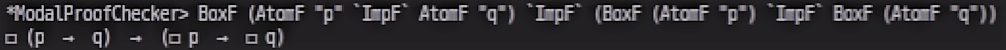
\includegraphics[width=\linewidth]{images/show_formula.png}
                \centering
                \caption{Exemplu de apel al funcției show pentru o formulă}
            \end{figure}

            \par{}
                În plus, nu este necesară scrierea axiomelor cel mai des întâlnite, deoarece pentru acestea sunt deja 
                definite variabile în cadrul modulului. Mai mult decât atât, sunt definite variabile și pentru cele 
                mai cunoscute sisteme de deducție, după cum se observă în următorul exemplu:

            \begin{lstlisting}
                axiom_k :: Formula
                axiom_k = BoxF (AtomF "p" `ImpF` AtomF "q") `ImpF` 
                         (BoxF (AtomF "p") `ImpF` BoxF (AtomF "q"))

                axiom_dual :: Formula
                axiom_dual = DiaF (AtomF "p") `EqvF` NotF (BoxF (NotF (AtomF "p")))

                axiom_4 :: Formula
                axiom_4 = BoxF (AtomF "p") `ImpF` BoxF (BoxF (AtomF "p"))
                
                system_k :: Deduction_System
                system_k = Axioms []

                system_k4 :: Deduction_System
                system_k4 = Axioms [axiom_4]
            \end{lstlisting}

            \par{}
                O listă completă a sistemelor de deducție implementate în cadrul modulului este următoarea: 
                \begin{itemize}
                    \item \texttt{system\_k} pentru orice tip de \textit{frame}
                    \item \texttt{system\_k4} pentru \textit{frame}-urile tranzitive
                    \item \texttt{system\_kt} pentru \textit{frame}-urile reflexive
                    \item \texttt{system\_kb} pentru \textit{frame}-urile euclidiene
                    \item \texttt{system\_kd} pentru \textit{frame}-urile seriale
                    \item \texttt{system\_kd45} pentru \textit{frame}-urile tranzitive, euclidiene și seriale
                    \item \texttt{system\_s4} pentru \textit{frame}-urile reflexive și tranzitive
                    \item \texttt{system\_s5} pentru \textit{frame}-urile a căror relație de accesibilitate este una 
                    de echivalență
                \end{itemize}
                Pot fi create și alte sisteme în afară de acestea, în funcție de necesități, iar în acest scop pot fi 
                folosite și axiomele oferite de modul. O listă completă a acestor axiome este următorarea:
                \begin{multicols}{3}
                    \noindent
                    \begin{itemize}
                        \item \texttt{axiom\_k}
                        \item \texttt{axiom\_dual}
                        \item \texttt{axiom\_4}
                        \item \texttt{axiom\_m}
                        \item \texttt{axiom\_d}
                        \item \texttt{axiom\_b}
                        \item \texttt{axiom\_5}
                        \item \texttt{axiom\_cd}
                        \item \texttt{axiom\_box\_m}
                        \item \texttt{axiom\_c4}
                        \item \texttt{axiom\_c}
                    \end{itemize}
                \end{multicols}
                Pentru o descriere mai detaliată a acestor axiome, se poate consulta 
                \mysectionreference{section_frame_classes}.
            
            \par{}
                Folosind aceste definiții, precum și exemplul de demonstrație prezentat la începutul acestei secțiuni 
                (\texttt{deductions\_example}), se poate construi o variabilă de tipul \texttt{Proof} care să 
                încapsuleze o demonstrație corectă.
            
            \begin{lstlisting}
                correct_proof :: Proof
                correct_proof = Proof system_k deductions_example
            \end{lstlisting}

            \begin{figure}[h!]
            \label{fig_verify_proof}
                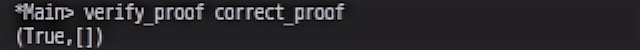
\includegraphics[width=.6\linewidth]{images/verify_proof.png}
                \centering
                \caption{Rezultatul funcției \texttt{verify\_proof} pentru o demonstrație corectă}
            \end{figure}

            \par{}
                Se poate observa în acest exemplu că pentru cazul unei demonstrații corecte este întors răspunsul 
                \texttt{True} pe prima poziție a perechii, iar pe a doua poziție este o listă vidă deoarece nu a fost 
                detectată nici o eroare. În cele ce urmează, vor fi introduse și câteva exemple de demonstrații care 
                conțin erori pentru a vedea răspunsul oferit de funcția \texttt{verify\_proof}. Pentru aceasta se 
                definesc următoarele două demonstrații:
            
            \begin{lstlisting}
                wrong_axiom_proof :: Proof
                wrong_axiom_proof = 
                    Proof system_k [(
                        axiom_k, 
                        KAxiom
                    ),(
                        axiom_4, 
                        DualAxiom
                    )]
                
                wrong_tautology_proof :: Proof
                wrong_tautology_proof = 
                    Proof system_k4 [(
                        NotF (AtomF "p") `OrF` AtomF "q", 
                        Taut
                    )]
                
                wrong_usub_proof :: Proof
                wrong_usub_proof = 
                    Proof system_k [(
                        AtomF "p" `OrF` NotF (AtomF "p"), 
                        Taut
                    ),(
                        AtomF "p" `OrF` NotF (AtomF "q"), 
                        US 1
                    )]
            \end{lstlisting}

            \par{}
                Primul dintre aceste exemple ilustrează o demonstrație în care este utilizată în mod greșit o axiomă. 
                Mai precis, este dedusă axioma tranzitivității ca fiind axioma duală. Următorul exemplu arată cazul 
                deducției unei formule ca fiind tautologie, deși formula dată nu este adevărată pentru orice evaluare.
                Ultimul exemplu reprezintă o aplicare greșită a substituției uniforme. Concret, greșeala constă în
                faptul că o apariție a atomului propozițional p este înlocuită cu atomul q, iar cealaltă 
                rămâne nemodificată. În continuare, este prezentată ieșirea pe care o produce funcția 
                \texttt{verify\_proof} în aceste două cazuri. 
            
            \begin{figure}[h]
            \label{fig_wrong_proof}
                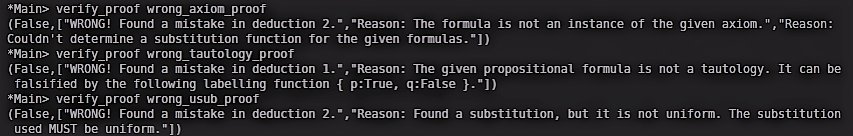
\includegraphics[width=\linewidth]{images/wrong_proof.png}
                \centering
                \caption{Rezultatul funcției \texttt{verify\_proof} pentru demonstrații greșite}
            \end{figure}

            \par{}
                Se poate observa că în toate cazurile este semnalat faptul că demonstrația este greșită prin valoarea 
                \texttt{False} de pe prima poziție a perechii returnate. Pe lista de pe poziția a doua se poate vedea că 
                în fiecare caz primul mesaj semnalează la ce deducție a fost detectată eroarea printr-un mesaj de forma 
                „WRONG! Found a mistake in deduction \textit{i}.” („INCORECT! Am găsit o greșeală în 
                deducția \textit{i}.”), numărul \textit{i} reprezentând numărul de ordine al formulei în cadrul demonstrației. 
                Acest mesaj este urmat de cel puțin un altul care detaliază motivul erorii. De accentuat este faptul 
                că pot apărea mai multe explicații, un astfel de exemplu fiind cazul deducției greșite a unei axiome, unde 
                sunt oferite mai multe detalii despre greșeala detectată. De asemenea, se poate vedea că pentru greșelile 
                în deducția tautologiilor este oferit și câte un exemplu de evaluare care invalidează proprietatea de 
                tautologie a acestora.
        % section Detalii pentru utilizare (end)
    % chapter Verificator de demonstrații (end)

    \chapter{Concluzii} % (fold)
    \label{chapter_conclusion}
        \section{Aprecieri critice} % (fold)
        \label{section_critical_appraisal}
            \par{}
                Această secțiune își propune să facă o analiză a modului în care a fost realizată a această lucrare, 
                expunând atât părțile pozitive precum și aspectele care ar putea fi îmbunătățite, cât și provocările 
                întâlnite. Totodată, se va urmări și în ce măsură au fost îndeplinite obiectivele propuse la 
                începutul acestei lucrări.
            
            \par{}
                Pentru început, atenția va fi concetrată asupra capitolul teoretic. În ceea ce privește prima parte a 
                lucrării, cel mai important aspect îl reprezintă conținutul acesteia. Din acest punct de vedere, 
                se poate considera că lucrarea și-a atins scopul ținând cont că au fost introduse conceptele de bază ale 
                logicii modale până la cele necesare demonstrațiilor sintactice în sistemele de tip Hilbert. Un alt plus 
                important al lucrării este reprezentat de exemplele prezentate de-a lungul acesteia. Chiar dacă numărul 
                acestora nu este mare, prin exemplele oferite au fost acoperite majoritatea noțiunilor prezentate. Mai 
                mult decât atât, în ultima secțiune, au fost detaliate și cazuri mai complexe de utilizare a logicii 
                modale, care pot oferi o idee asupra importanței acesteia. Un punct important ce a fost atins este 
                accesibilitatea, deoarece chiar și în contextul exemplelor mai complexe, au fost aduse explicații 
                cuprinzătoare.
            
            \par{}
                Un alt aspect ce trebuie luat în considerare, în evaluarea redactării capitolului teoretic este 
                structura acestuia. Structurarea ideilor a reprezentat un pas important în elaborarea lucrării și ar 
                trebui considerat astfel pentru orice tip de lucrare indiferent de scopul acesteia. Din punct de vedere 
                structural, se remarcă ca aspect pozitiv alegerea de a prezenta în prima partea a capitolului logica 
                modală de bază, fapt ce, fără nici un dubiu, a condus la o lucrarea mult mai ușor de urmărit, elementele 
                noi fiind introduse gradual. De asemenea,un element imporant este reprezentat și de faptul că 
                prezentarea unei secțiuni cu exemple de interpretări ale logicii modale de bază (secțiunea 4) a fost 
                realizată cât mai devreme în lucrare (imediat după introducerea sintaxei și a semanticii) pentru a putea 
                construi o intuiție cititorului asupra rolului pe care îl au operatorii modali. Se poate spune că unele 
                idei prezentate ar putea fi dezvoltate mai mult, însă ținând cont de aspectele expuse anterior, cât și 
                de dimensiunile capitolului teoretic raportat la complexitatea temei abordate, se poate concluzia că 
                rezultatul obținut este foarte bun și relevant.
            
            \par{}
                În cele ce urmează, se va face referire la exemplul practic atât la etapele dezvoltării, cât și la 
                documentarea acestuia. În ceea ce privește implementarea, cel mai important pas a fost modelarea 
                conceptelor logice necesare. Odată ce acesta a fost definitivat într-o manieră convenabilă, o mare parte 
                a implementării a decurs în mod natural. Un alt punct important în dezvoltarea modulului a fost 
                reprezentat de oferirea de explicații cât mai clare în cazul detectării erorilor. Pentru aceasta, poate 
                fi considerată inspirată alegerea utilizării monadei \texttt{Writer}, care a permis atingerea acestui 
                țel fără a afecta foarte mult structura codului. Făcând trecerea la perspectiva unui utilizator al 
                modulului, acesta ar trebui să fie destul de accesibil pentru o persoană ce posedă cunoștințe de bază 
                ale limbajului Haskell. Totuși, un aspect ce ar putea fi îmbunătățit este legat de introducerea 
                formulelor, care pot deveni destul de complexe și greu de scris utilizând constructori definiți, care nu
                se aseamănă cu simboluri logice și pot deveni dificil de urmărit. Pentru a rezolva acest incovenient, se 
                poate implementa un \textit{parser} pentru expresii ce ar permite atât utilizarea unor simboluri mai 
                sugestive pentru operatorii logici, cât și creșterea accesibilității acestui modul, oferind 
                posibilitatea utilizării acestuia și de către persoanele ce nu au cunoștințe de Haskell. Însă, această 
                sarcină ar fi fost destul de consumatoare de timp și avantajul oferit nu ar fi fost unul consistent în 
                contextul acestei lucrări, reușindu-se o ameliorare a problemei prin implementarea metodei de printare a 
                formulelor care poate înlocui parțial un \textit{parser}.

            \par{}
                În ceea ce privește redactarea capitolului practic, chiar dacă exemplul prezentat a fost realizat în 
                limbajul Haskell, explicațiile oferite pentru implementarea modulului nu s-au rezumat doar la 
                particularități ale limbajului, ci s-a încercat o prezentare a funcționalității accesibilă și unei 
                persoane fără cunoștințe de programare în Haskell. Din acest punct de vedere, prezentarea a fost 
                reușită, deși \mysectionreference{section_data_type} dedicată tipurilor de date, care are o importanță 
                deosebită pentru înțelegerea implementării, se poate dovedi a fi mai dificil de urmărit pentru o 
                persoană care nu are experiență cu utilizarea acestui limbaj. Din perspectiva modului de 
                utilizare, sunt expuse toate detaliile necesare și, în plus, acestea sunt ilustrate cu exemple 
                edificatoare.
            
            \par{}
                Punând la un loc toate ideile prezentate anterior, se poate spune că lucrarea de față și-a atins 
                obiectivele setate la început, reprezentând un punct de plecare pentru o persoană care dorește să 
                descopere ce este logica modală sau dorește să afle cum pot fi aplicate conceptele logicii modale în 
                programare.
        % section Aprecieri critice (end)

        \section{Posibile dezvoltări} % (fold)
        \label{section_future_work}
            \par{}
                În privința dezvoltărilor viitoare, discuția poate fi, și aici, împărțită în funcție de cele două 
                direcții importante ale lucrării, cea practică și cea teoretică. Din punctul de vedere al aplicației, ar 
                fi interesantă dezvoltarea verificatorului de demonstrații pentru a permite compatibilitate completă cu 
                logica modală și nu doar cu cea de bază (cum este la momentul actual). Pentru aceasta, trecerea la un 
                număr finit de operatori modali cu diferite arități nu ar trebuie să se realizeze foarte dificil. Însă, 
                modelarea unei probleme cum ar fi cea a logicii propoziționale dinamice, a cărei definiție permite un 
                număr infinit de mare de operatori și ale cărei axiome sunt de asemenea infinit de multe, ar reprezenta 
                fără îndoială o provocare. De asemenea, trebuie menționată ca posibilă îmbunătățire și ideea punctată în
                secțiunea anterioară referitoare la implementarea unei modalități mai simple de introducere a 
                formulelor sub forma unui \textit{parser}.

            \par{}
                În ceea ce privește dezvoltările părții teoretice, ținând cont de generalitatea logicii modale studierea 
                acesteia permite deschiderea către multe alte domenii de studiu. Dintre acestea, merită menționată 
                logica dinamică, care se bazează pe logica modală. Aceasta ajută la modelarea execuției programelor și 
                la verificarea corectitudinii acestora. De asemenea, un alt domeniu de studiu interesant poate fi 
                reprezentat de construcția demonstratoarelor pentru astfel de tipuri de logică. Principală deosebire 
                dintre un verificator de demonstrații și un demonstrator este că scopul celui din urmă este de a 
                determina dacă o formulă este validă sau nu, fără a primi pașii pe care trebuie să-i urmeze.
        % section Posibile dezvoltări (end)
    % chapter Concluzii (end)

    \selectbiblanguage{romanian}
    \bibliographystyle{plain}
    \bibliography{bibliografie.bib} % Adauga fisierul cu bibliografia
    \addcontentsline{toc}{chapter}{Bibliografie}
\end{document}
